% \documentclass[a4paper,dvipsnames]{article}

% \addtolength{\hoffset}{-2.25cm}
% \addtolength{\textwidth}{4.5cm}
% \addtolength{\voffset}{-3.25cm}
% \addtolength{\textheight}{5cm}
% \setlength{\parskip}{0pt}
% \setlength{\parindent}{0in}

% %----------------------------------------------------------------------------------------
%	PACKAGES AND OTHER DOCUMENT CONFIGURATIONS
%----------------------------------------------------------------------------------------

%----------------------------------------------------------------------------------------
%		Generals
%----------------------------------------------------------------------------------------
\usepackage{fourier}
\usepackage{frcursive}
\usepackage[T1]{fontenc} %Accents handling
\usepackage[utf8]{inputenc} % Use UTF-8 encoding
%\usepackage{microtype} % Slightly tweak font spacing for aesthetics
\usepackage[english, francais]{babel} % Language hyphenation and typographical rules

%----------------------------------------------------------------------------------------
%		Graphics
%----------------------------------------------------------------------------------------
\usepackage{xcolor}
\usepackage{graphicx, multicol} % Enhanced support for graphics
\graphicspath{{FIG/}}
\usepackage{wrapfig}

%----------------------------------------------------------------------------------------
%		Other packages
%----------------------------------------------------------------------------------------
\usepackage{hyperref}
\hypersetup{
	colorlinks=true, %colorise les liens
	breaklinks=true, %permet le retour à la ligne dans les liens trop longs
	urlcolor= bleu3,  %couleur des hyperliens
	linkcolor= bleu3, %couleur des liens internes
	plainpages=false  %pour palier à "Bookmark problems can occur when you have duplicate page numbers, for example, if you have a page i and a page 1."
}
\usepackage{tabularx}
\newcolumntype{M}[1]{>{\arraybackslash}m{#1}} %Defines a scalable column type in tabular
\usepackage{booktabs} % Enhances quality of tables
\usepackage{diagbox} % barre en diagonale dans un tableau
\usepackage{multicol}
\usepackage[explicit]{titlesec}


%----------------------------------------------------------------------------------------
%		Headers and footers
%----------------------------------------------------------------------------------------
\usepackage{fancyhdr} % Headers and footers
\pagestyle{fancy} % All pages have headers and footers
\fancyhead{}\renewcommand{\headrulewidth}{0pt} % Blank out the default header
\renewcommand{\footrulewidth}{0pt}
\fancyfoot[L]{} % Custom footer text
\fancyfoot[C]{\href{https://sacado.xyz/}{sacado.xyz}} % Custom footer text
\fancyfoot[R]{\thepage} % Custom footer text

%----------------------------------------------------------------------------------------
%		Mathematics packages
%----------------------------------------------------------------------------------------
\usepackage{amsthm, amsmath, amssymb} % Mathematical typesetting
\usepackage{marvosym, wasysym} % More symbols
\usepackage[makeroom]{cancel}
\usepackage{xlop}
\usepackage{pgf,tikz,pgfplots}
\pgfplotsset{compat=1.15}
\usetikzlibrary{positioning}
%\usetikzlibrary{arrows}
\usepackage{pst-plot,pst-tree,pst-func, pstricks-add,pst-node,pst-text}
\usepackage{units}
\usepackage{nicefrac}
\usepackage[np]{numprint} %Séparation milliers dans un nombre

%----------------------------------------------------------------------------------------
%		New text commands
%----------------------------------------------------------------------------------------
\usepackage{calc}
\usepackage{boites}
 \renewcommand{\arraystretch}{1.6}

%%%%% Pour les imports.
\usepackage{import}

%%%%% Pour faire des boites
\usepackage[tikz]{bclogo}
\usepackage{bclogo}
\usepackage{framed}
\usepackage[skins]{tcolorbox}
\tcbuselibrary{breakable}
\tcbuselibrary{skins}
\usetikzlibrary{babel,arrows,shadows,decorations.pathmorphing,decorations.markings,patterns}

%%%%% Pour les symboles et les ensembles
\newcommand{\pp}{\leq}
\newcommand{\pg}{\geq}
%\newcommand{\euro}{\eurologo{}}
\newcommand{\R}{\mathbb{R}}
\newcommand{\N}{\mathbb{N}}
\newcommand{\D}{\mathbb{D}}
\newcommand{\Z}{\mathbb{Z}}
\newcommand{\Q}{\mathbb{Q}}
\newcommand{\C}{\mathbb{C}}

%%%%% Pour une double minipage
\newcommand{\mini}[2]{
\begin{minipage}[t]{0.48\linewidth}
#1
\end{minipage}
\hfill
\begin{minipage}[t]{0.48\linewidth}
#2
\end{minipage}
}


%\newcommand\hole[1]{\texttt{\_}}
%\newcommand{\PROP}[1]{\textbf{\underline{#1}}}
%\newcommand{\exercice}{\textcolor{OliveGreen}{Exercice : }}
%\newcommand{\correction}{\textcolor{BurntOrange}{Correction : }}
%\newcommand{\propriete}{\textbf{\underline{Propriété}} : }
%\newcommand{\prop}{\textbf{\underline{Propriété}} : }
%\newcommand{\vocabulaire}{\textbf{\underline{Vocabulaire}} : }
%\newcommand{\voca}{\textbf{\underline{Vocabulaire}} : }

\usepackage{enumitem}
\newlist{todolist}{itemize}{2} %Pour faire des QCM
\setlist[todolist]{label=$\square$} %Pour faire des QCM \begin{todolist} instead of itemize

%----------------------------------------------------------------------------------------
%		Définition de couleur pour geogebra
%----------------------------------------------------------------------------------------
\definecolor{zzttqq}{rgb}{0.6,0.2,0.} %rouge des polygones
\definecolor{qqqqff}{rgb}{0.,0.,1.}
\definecolor{xdxdff}{rgb}{0.49019607843137253,0.49019607843137253,1.}%bleu
\definecolor{qqwuqq}{rgb}{0.,0.39215686274509803,0.} %vert des angles
\definecolor{ffqqqq}{rgb}{1.,0.,0.} %rouge vif
\definecolor{uuuuuu}{rgb}{0.26666666666666666,0.26666666666666666,0.26666666666666666}
\definecolor{qqzzqq}{rgb}{0.,0.6,0.}
\definecolor{cqcqcq}{rgb}{0.7529411764705882,0.7529411764705882,0.7529411764705882} %gris
\definecolor{qqffqq}{rgb}{0.,1.,0.}
\definecolor{ffdxqq}{rgb}{1.,0.8431372549019608,0.}
\definecolor{ffffff}{rgb}{1.,1.,1.}
\definecolor{ududff}{rgb}{0.30196078431372547,0.30196078431372547,1.}

%-------------------------------------------------
%
%	EN TETE
%
%-------------------------------------------------

% Classe
\newcommand{\myClasse}   
{
    6e
}

% Discipline
\newcommand{\myDiscipline}   
{
    Mathématiques
}

% Parcours
\newcommand{\myParcours}
{
  Nombres et Calculs
}

%Titre de la séquence
\newcommand{\myTitle}
{
    \scshape\huge
\textcolor{sacado_purple}{
		Nombres décimaux
}
}

%----------------------------------------------------------------------------------------

% %----------------------------------------------------------------------------------------
%		Définition de couleur pour les boites
%----------------------------------------------------------------------------------------
\definecolor{bleu1}{rgb}{0.54,0.79,0.95} %% Bleu
\definecolor{sapgreen}{rgb}{0.4, 0.49, 0}
\definecolor{dvzfxr}{rgb}{0.7,0.4,0.}
\definecolor{beamer}{rgb}{0.5176470588235295,0.49019607843137253,0.32941176470588235} % couleur beamer
\definecolor{preuveRbeamer}{rgb}{0.8,0.4,0}
\definecolor{sectioncolor}{rgb}{0.24,0.21,0.44}
\definecolor{subsectioncolor}{rgb}{0.1,0.21,0.61}
\definecolor{subsubsectioncolor}{rgb}{0.1,0.21,0.61}
\definecolor{info}{rgb}{0.82,0.62,0}
\definecolor{bleu2}{rgb}{0.38,0.56,0.68}
\definecolor{bleu3}{rgb}{0.24,0.34,0.40}
\definecolor{bleu4}{rgb}{0.12,0.20,0.25}
\definecolor{vert}{rgb}{0.21,0.33,0}
\definecolor{vertS}{rgb}{0.05,0.6,0.42}
\definecolor{red}{rgb}{0.78,0,0}
\definecolor{color5}{rgb}{0,0.4,0.58}
\definecolor{eduscol4B}{rgb}{0.19,0.53,0.64}
\definecolor{eduscol4P}{rgb}{0.62,0.12,0.39}

%----------------------------------------------------------------------------------------
%		Définition de couleur pour les boites SACADO
%----------------------------------------------------------------------------------------
\definecolor{sacado_blue}{RGB}{0,129,159} %% Bleu Sacado
\definecolor{sacado_green}{RGB}{59, 157, 38} %% Vert Sacado
\definecolor{sacado_yellow}{RGB}{255,180,0} %% Jaune Sacado
\definecolor{sacado_purple}{RGB}{94,68,145} %% Violet foncé Sacado
\definecolor{sacado_violet}{RGB}{153,117,224} %% Violet clair Sacado
\definecolor{sacado_orange}{RGB}{249,168,100} %% Orange Sacado
\definecolor{ill_frame}{HTML}{F0F0F0}
\definecolor{ill_back}{HTML}{F7F7F7}
\definecolor{ill_title}{HTML}{AAAAAA}


 % Compteurs pour Théorème, Définition, Exemple, Remarque, .....
\newcounter{cpttheo}
\setcounter{cpttheo}{0}
\newcounter{cptdef}
\setcounter{cptdef}{0}
\newcounter{cptmth}
\setcounter{cptmth}{0}
\newcounter{cpttitre}
\setcounter{cpttitre}{0}
 % Exercices
\newcounter{cptapp}
\setcounter{cptapp}{0}
\newcounter{cptex}
\setcounter{cptex}{0}
\newcounter{cptsr}
\setcounter{cptsr}{0}
\newcounter{cpti}
\setcounter{cpti}{0}
\newcounter{cptcor}
\setcounter{cptcor}{0}




%%%%% Pour réinitialiser numéros des paragraphes après une nouvelle partie
\makeatletter
    \@addtoreset{paragraph}{part}
\makeatother


%%%% Titres et sections

\newlength\chapnumb
\setlength\chapnumb{3cm}


% \titleformat{\part}[block] {
 % \normalfont\sffamily\color{violet}}{}{0pt} {
   % \parbox[t]{\chapnumb}{\fontsize{120}{110}\selectfont\ding{110}}
   % \parbox[b]{\dimexpr\textwidth-\chapnumb\relax}{
       % \raggedleft
       % \hfill{{\color{bleu3}\fontsize{40}{30}\selectfont#1}}\\
       % \rule{0.99\textwidth-\chapnumb\relax}{0.4pt}
 % }
% }

% \titleformat{name=\part,numberless}[block]
% {\normalfont\sffamily\color{bleu3}}{}{0pt}
% {\parbox[b]{\chapnumb}{%
  % \mbox{}}%
 % \parbox[b]{\dimexpr\textwidth-\chapnumb\relax}{%
   % \raggedleft%
   % \hfill{{\color{bleu3}\fontsize{40}{30}\selectfont#1}}\\
   % \rule{0.99\textwidth-\chapnumb\relax}{0.4pt}
 % }
% }



% \titleformat{\chapter}[block] {
 % \normalfont\sffamily\color{violet}}{}{0pt} {
   % \parbox[t]{\chapnumb}{ 
     % \fontsize{120}{110}\selectfont\thechapter}
     % \parbox[b]{\textwidth-\chapnumb}{
       % \raggedleft
       % \hfill{{\color{bleu3}\huge#1}}\\  
  % \ifthenelse{\thechapter<10}{\rule{0.99\textwidth-\chapnumb}{0.4pt}}{\rule{0.9\textwidth - \chapnumb}{0.4pt}}
       % \setcounter{cpttitre}{0}
	% \setcounter{cptapp}{0}
	% \setcounter{cptex}{0}
	% \setcounter{cptsr}{0}
	% \setcounter{cpti}{0}
	% \setcounter{cptcor}{0} 
 % }
% }

% \titleformat{name=\chapter,numberless}[block]
% {\normalfont\sffamily\color{bleu3}}{}{0pt}
% {\parbox[b]{\chapnumb}{%
  % \mbox{}}%
 % \parbox[b]{\textwidth-\chapnumb}{%
   % \raggedleft
   % \hfill{{\color{bleu3}\huge#1}}\\
   % \ifthenelse{\thechapter<10}{\rule{0.99\textwidth-\chapnumb}{0.4pt}}{ \rule{0.9\textwidth - \chapnumb}{0.4pt}}
       % \setcounter{cpttitre}{0}
	% \setcounter{cptapp}{0}
	% \setcounter{cptex}{0}
	% \setcounter{cptsr}{0}
	% \setcounter{cpti}{0}
	% \setcounter{cptcor}{0} 
 % }
% }
%
%       
%
%%%%% Personnalisation des numéros des sections
\renewcommand\thesection{\Roman{section}. }
\renewcommand\thesubsection{\hspace{1cm}\arabic{subsection}. }
\renewcommand\thesubsubsection{\hspace{2cm}\alph{subsubsection}. }

\titleformat{\section}[hang]{\color{sacado_purple}{}\normalfont\filright\huge}{}{0.4em}{\textbf{\thesection  #1}}   
% \titlespacing*{\section}{0.2pt}{0ex plus 0ex minus 0ex}{0.3em}
   
\titleformat{\subsection}[hang]{\color{sacado_purple}{}\normalfont\filright\Large}{}{0.4em}{\thesubsection
 #1}            
\titleformat{\subsubsection}[hang]{\color{sacado_purple}{}\normalfont\filright\large}{}{0.4em}{\thesubsubsection
 #1}
\titleformat{\paragraph}[hang]{\color{black}{}\normalfont\filright\normalsize}{}{0.4em}{#1}



%%%%%%%%%%%%%%%%%%%%% Cycle 4
%\newcommand{\Titre}[2]{\section*{#1 
%\ifthenelse{\equal{#2}{1}}   {\hfill{ \ding{182}  \ding{173} \ding{174} } \addcontentsline{toc}{section}{#1 \ding{182}} }%
%{%
%\ifthenelse{\equal{#2}{2}}{\hfill{ \ding{172}  \ding{183} \ding{174} } \addcontentsline{toc}{section}{#1 {\color{purple}\ding{183}}} }{%           
%\hfill{ \ding{172}  \ding{173} \ding{184} } \addcontentsline{toc}{section}{#1 {\color{orange}\ding{184}}}% 
%}%
%}%
%}
%}


%%%%%%%%%%%%%%%%%%%%% Cycle 4
\newcommand{\Titre}[2]{\section*{#1 
\ifthenelse{\equal{#2}{1}}   {\hfill{ \ding{182}  \ding{173} \ding{174} } \addcontentsline{toc}{section}{#1 \, \ding{182}} }%
{% sinon
\ifthenelse{\equal{#2}{1,5}}   {\hfill{ \ding{182}  \ding{183} \ding{174} } \addcontentsline{toc}{section}{#1 \, \ding{182} {\color{purple}\ding{183}}} }%
{% sinon
\ifthenelse{\equal{#2}{2}}   {\hfill{ \ding{172}  \ding{183} \ding{174} } \addcontentsline{toc}{section}{#1 \, {\color{purple}\ding{183}}} }
{% sinon
\ifthenelse{\equal{#2}{2,5}}   {\hfill{ \ding{172}  \ding{183} \ding{184} } \addcontentsline{toc}{section}{#1 \, {\color{purple}\ding{183}}  {\color{orange}\ding{184}}} }%
{% sinon
\hfill{ \ding{172}  \ding{173} \ding{184} } \addcontentsline{toc}{section}{#1 \,{\color{orange}\ding{184}}}% 
}%
}%
}%
}%
}%
}

%%%%%%%%%%%%% Titre
\newenvironment{titre}[2][]{%
\vspace{0.5cm}
\begin{tcolorbox}[enhanced, lifted shadow={0mm}{0mm}{0mm}{0mm}%
{black!60!white}, attach boxed title to top left={xshift=110mm, yshift*=-3mm}, coltitle=violet, colback=bleu3!25!white, boxed title style={colback=white!100}, colframe=bleu3,title=\stepcounter{cpttitre} \textbf{Fiche \thecpttitre}. #1 #2 ]}
{%
\end{tcolorbox}
\par}



%%%%%%%%%%%%% Définitions
\newenvironment{Def}[1][]{%
\medskip \begin{tcolorbox}[widget,colback=sacado_violet!0,colframe=sacado_violet!75,
adjusted title= \stepcounter{cptdef} Définition \thecptdef . {#1} ]}
{%
\end{tcolorbox}\par}


\newenvironment{DefT}[2][]{%
\medskip \begin{tcolorbox}[widget,colback=sacado_violet!0,colframe=sacado_violet!75,
adjusted title= \stepcounter{cptdef} Définition \thecptdef . {#1} \textit{#2}]}
{%
\end{tcolorbox}\par}

%%%%%%%%%%%%% Proposition
\newenvironment{Prop}[1][]{%
\medskip \begin{tcolorbox}[widget,colback=sacado_blue!0,colframe=sacado_blue!75!black,
adjusted title= \stepcounter{cpttheo} Proposition \thecpttheo . {#1} ]}
{%
\end{tcolorbox}\par}

%%%%%%%%%%%%% Propriétés
\newenvironment{Pp}[1][]{%
\medskip \begin{tcolorbox}[widget,colback=sacado_blue!0,colframe=sacado_blue!75!black,
adjusted title= \stepcounter{cpttheo} Propriété \thecpttheo . {#1}]}
{%
\end{tcolorbox}\par}

\newenvironment{PpT}[2][]{%
\medskip \begin{tcolorbox}[widget,colback=sacado_blue!0,colframe=sacado_blue!75!black,
adjusted title= \stepcounter{cpttheo} Propriété \thecpttheo . {#1} #2]}
{%
\end{tcolorbox}\par}

\newenvironment{Pps}[1][]{%
\medskip \begin{tcolorbox}[widget,colback=sacado_blue!0,colframe=sacado_blue!75!black,
adjusted title= \stepcounter{cpttheo} Propriétés \thecpttheo . {#1}]}
{%
\end{tcolorbox}\par}

%%%%%%%%%%%%% Théorèmes
\newenvironment{ThT}[2][]{% théorème avec titre
\medskip \begin{tcolorbox}[widget,colback=sacado_blue!0,colframe=sacado_blue!75!black,
adjusted title= \stepcounter{cpttheo} Théorème \thecpttheo . {#1} #2]}
{%
\end{tcolorbox}\par}

\newenvironment{Th}[1][]{%
\medskip \begin{tcolorbox}[widget,colback=sacado_blue!0,colframe=sacado_blue!75!black,
adjusted title= \stepcounter{cpttheo} Théorème \thecpttheo . {#1}]}
{%
\end{tcolorbox}\par}

%%%%%%%%%%%%% Règles
\newenvironment{Reg}[1][]{%
\medskip \begin{tcolorbox}[widget,colback=sacado_blue!0,colframe=sacado_blue!75!black,
adjusted title= \stepcounter{cpttheo} Règle \thecpttheo . {#1}]}
{%
\end{tcolorbox}\par}

%%%%%%%%%%%%% REMARQUES
\newenvironment{Rq}[1][]{%
\begin{bclogo}[couleur=sacado_orange!0, arrondi =0.15, noborder=true, couleurBarre=sacado_orange, logo = \bcinfo ]{ 
{\color{info}\normalsize{Remarque#1}}}}
{%
\end{bclogo}
\par}


\newenvironment{Rqs}[1][]{%
\begin{bclogo}[couleur=sacado_orange!0, arrondi =0.15, noborder=true, couleurBarre=sacado_orange, logo = \bcinfo ]{ 
{\color{info}\normalsize{Remarques#1}}}}
{%
\end{bclogo}
\par}

%%%%%%%%%%%%% EXEMPLES
\newenvironment{Ex}[1][]{%
\begin{bclogo}[couleur=sacado_yellow!15, arrondi =0.15, noborder=true, couleurBarre=sacado_yellow, logo = \bclampe ]{ 
\normalsize{Exemple#1}}}
{%
\end{bclogo}
\par}




%%%%%%%%%%%%% Preuve
\newenvironment{Pv}[1][]{%
\begin{tcolorbox}[breakable, enhanced,widget, colback=sacado_blue!10!white,boxrule=0pt,frame hidden,
borderline west={1mm}{0mm}{sacado_blue!75}]
\textbf{Preuve#1 : }}
{%
\end{tcolorbox}
\par}


%%%%%%%%%%%%% PreuveROC
\newenvironment{PvR}[1][]{%
\begin{tcolorbox}[breakable, enhanced,widget, colback=sacado_blue!10!white,boxrule=0pt,frame hidden,
borderline west={1mm}{0mm}{sacado_blue!75}]
\textbf{Preuve (ROC)#1 : }}
{%
\end{tcolorbox}
\par}


%%%%%%%%%%%%% Compétences
\newenvironment{Cps}[1][]{%
\vspace{0.4cm}
\begin{tcolorbox}[enhanced, lifted shadow={0mm}{0mm}{0mm}{0mm}%
{black!60!white}, attach boxed title to top left={xshift=5mm, yshift*=-3mm}, coltitle=white, colback=white, boxed title style={colback=sacado_green!100}, colframe=sacado_green!75!black,title=\textbf{Compétences associées#1}]}
{%
\end{tcolorbox}
\par}

%%%%%%%%%%%%% Compétences Collège
\newenvironment{CpsCol}[1][]{%
\vspace{0.4cm}
\begin{tcolorbox}[breakable, enhanced,widget, colback=white ,boxrule=0pt,frame hidden,
borderline west={2mm}{0mm}{bleu3}]
\textbf{#1}}
{%
\end{tcolorbox}
\par}




%%%%%%%%%%%%% Attendus
\newenvironment{Ats}[1][]{%
\vspace{0.4cm}
\begin{tcolorbox}[enhanced, lifted shadow={0mm}{0mm}{0mm}{0mm}%
{black!60!white}, attach boxed title to top left={xshift=5mm, yshift*=-3mm}, coltitle=white, colback=white, boxed title style={colback=sacado_green!100}, colframe=sacado_green!75!black,title=\textbf{Attendus du chapitre#1}]}
{%
\end{tcolorbox}
\par}

%%%%%%%%%%%%% Méthode
\newenvironment{Mt}[1][]{%
\vspace{0.4cm}
\begin{bclogo}[couleur=sacado_blue!0, arrondi =0.15, noborder=true, couleurBarre=bleu3, logo = \bccrayon ]{ 
\normalsize{{\color{bleu3}Méthode #1}}}}
{%
\end{bclogo}
\par}


%%%%%%%%%%%%% Méthode en vidéo
\newcommand{\MtV}[2]{\vspace{0.4cm} \colorbox{sacado_blue!0}{\hspace{0.2 cm}\tikz\node[rounded corners=1pt,draw] {\color{red}$\blacktriangleright$}; \quad  \href{https://youtu.be/#1?rel=0}{\raisebox{0.8mm}{{\color{red}\textbf{Méthode en vidéo : #2}}}}}}


%%%%%%%%%%%%% A voir (AV) : Lien externe + vidéo non Youtube
\newcommand{\AV}[2]{\vspace{0.4cm} \colorbox{bleu1!0}{\hspace{0.2 cm}\tikz\node[rounded corners=1pt,draw] {\color{red}$\blacktriangleright$}; \quad  \href{#1}{\raisebox{0.8mm}{{\color{red}\textbf{#2}}}}}}


%%%%%%%%%%%%% Etymologie
\newenvironment{Ety}[1][]{%
\begin{bclogo}[couleur=sacado_green!0, arrondi =0.15, noborder=true, couleurBarre=sacado_green, logo = \bcplume ]{ 
\normalsize{{\color{sacado_green}Étymologie#1}}}}
{%
\end{bclogo}
\par}


%%%%%%%%%%%%% Notation
\newenvironment{Nt}[1][]{%
\begin{bclogo}[couleur=sacado_violet!0, arrondi =0.15, noborder=true, couleurBarre=sacado_violet!75, logo = \bccrayon ]{ 
\normalsize{{\color{violet!75}Notation#1}}}}
{%
\end{bclogo}
\par}
%%%%%%%%%%%%% Histoire
%\newenvironment{His}[1][]{%
%\begin{bclogo}[couleur=brown!30, arrondi =0.15, noborder=true, couleurBarre=brown, logo = \bcvaletcoeur ]{ 
%\normalsize{{\color{brown}Histoire des mathématiques#1}}}}
%{%
%\end{bclogo}
%\par}

\newenvironment{His}[1][]{%
\vspace{0.4cm}
\begin{tcolorbox}[enhanced, lifted shadow={0mm}{0mm}{0mm}{0mm}%
{brown!60!white}, attach boxed title to top left={xshift=5mm, yshift*=-3mm}, coltitle=white, colback=white, boxed title style={colback=brown!100}, colframe=brown!75!black,title=\textbf{Histoire des mathématiques#1}]}
{%
\end{tcolorbox}
\par}

%%%%%%%%%%%%% Attention
\newenvironment{Att}[1][]{%
\begin{bclogo}[couleur=red!0, arrondi =0.15, noborder=true, couleurBarre=red, logo = \bcattention ]{ 
\normalsize{{\color{red}Attention. #1}}}}
{%
\end{bclogo}
\par}


%%%%%%%%%%%%% Conséquence
\newenvironment{Cq}[1][]{%
\textbf{Conséquence #1}}
{%
\par}

%%%%%%%%%%%%% Vocabulaire
\newenvironment{Voc}[1][]{%
\setlength{\logowidth}{10pt}
%\begin{footnotesize}
\begin{bclogo}[ noborder , couleur=white, logo =\bcbook]{#1}}
{%
\end{bclogo}
%\end{footnotesize}
\par}


%%%%%%%%%%%%% Video
\newenvironment{Vid}[1][]{%
\setlength{\logowidth}{12pt}
\begin{bclogo}[ noborder , couleur=white,barre=none, logo =\bcoeil]{#1}}
{%
\end{bclogo}
\par}


%%%%%%%%%%%%% Syntaxe
\newenvironment{Syn}[1][]{%
\begin{bclogo}[couleur=violet!0, arrondi =0.15, noborder=true, couleurBarre=violet!75, logo = \bcicosaedre ]{ 
\normalsize{{\color{violet!75}Syntaxe#1}}}}
{%
\end{bclogo}
\par}

%%%%%%%%%%%%% Auto évaluation
\newenvironment{autoeval}[1][]{%
\vspace{0.4cm}
\begin{tcolorbox}[enhanced, lifted shadow={0mm}{0mm}{0mm}{0mm}%
{black!60!white}, attach boxed title to top left={xshift=5mm, yshift*=-3mm}, coltitle=white, colback=white, boxed title style={colback=sacado_green!100}, colframe=sacado_green!75!black,title=\textbf{J'évalue mes compétences#1}]}
{%
\end{tcolorbox}
\par}


\newenvironment{autotest}[1][]{%
\vspace{0.4cm}
\begin{tcolorbox}[enhanced, lifted shadow={0mm}{0mm}{0mm}{0mm}%
{red!60!white}, attach boxed title to top left={xshift=5mm, yshift*=-3mm}, coltitle=white, colback=white, boxed title style={colback=red!100}, colframe=red!75!black,title=\textbf{Pour faire le point #1}]}
{%
\end{tcolorbox}
\par}

\newenvironment{ExOApp}[1][]{% Exercice d'application direct
\vspace{0.4cm}
\begin{tcolorbox}[enhanced, lifted shadow={0mm}{0mm}{0mm}{0mm}%
{red!60!white}, attach boxed title to top left={xshift=5mm, yshift*=-3mm}, coltitle=white, colback=white, boxed title style={colback=sacado_green!100}, colframe=sacado_green!75!black,title=\textbf{Application #1}]}
{%
\end{tcolorbox}
\par}

\newenvironment{ExOInt}[1][]{% Exercice d'application direct
\vspace{0.4cm}
\begin{tcolorbox}[enhanced, lifted shadow={0mm}{0mm}{0mm}{0mm}%
{red!60!white}, attach boxed title to top left={xshift=5mm, yshift*=-3mm}, coltitle=white, colback=white, boxed title style={colback=sacado_green!50}, colframe=sacado_green!75!black,title=\textbf{Exercice #1}]}
{%
\end{tcolorbox}
\par}

%Illustrations
\newtcolorbox{Illqr}[1]{
  enhanced,
  colback=white,
  colframe=ill_frame,
  colbacktitle=ill_back,
  coltitle=ill_title,
  title=\textbf{Illustration},
  boxrule=1pt, % épaisseur du trait à 1pt
  center,
  overlay={
    \node[anchor=south east, inner sep=0pt,xshift=-1pt,yshift=2pt,fill=white] at (frame.south east) {\fancyqr[height=1cm]{#1}};
  },
  after=\par,
  before=\vspace{0.4cm},
}

\newtcolorbox{Ill}{
  enhanced,
  colback=white,
  colframe=ill_frame,
  colbacktitle=ill_back,
  coltitle=ill_title,
  title=\textbf{Illustration},
  boxrule=1pt, % épaisseur du trait à 1pt
  center,
  after=\par,
  before=\vspace{0.4cm},
}

%%%%%%%%%%%%%% Propriétés
%\newenvironment{Pp}[1][]{%
%\medskip \begin{tcolorbox}[widget,colback=sacado_blue!0,colframe=sacado_blue!75!black,
%adjusted title= \stepcounter{cpttheo} Propriété \thecpttheo . {#1}]}
%{%
%\end{tcolorbox}\par}

%%%%% Pour réinitialiser numéros des chapitres après une nouvelle partie
% \makeatletter
    % \@addtoreset{section}{part}
% \makeatother

% \newcommand{\EPC}[3]{ % Exercice par compétence de niveau 1
% \ifthenelse{\equal{#1}{1}}
% {%condition2 vraie
% \vspace{0.4cm}
% \stepcounter{cptex}
% \tikz\node[rounded corners=0pt,draw,fill=bleu2]{\color{white}\textbf{ \thecptex}}; \quad  {\color{bleu2}\textbf{#3}}
% \input{#2}
% }% fin condition2 vraie
% {%condition2 fausse
% \vspace{0.4cm}
% \stepcounter{cptex}
% \tikz\node[rounded corners=2pt,draw,fill=eduscol4P]{\color{white}\textbf{ \thecptex}}; \quad  {\color{eduscol4P} \textbf{En temps libre.} \textbf{ #3}} 
% \input{#2}
% }% fin condition2 fausse
% } % fin de la procédure

% \usepackage{hyperref}

% \begin{document}

%-------------------------------
%	TITLE SECTION
%-------------------------------

% \fancyhead[C]{}
% \hrule\medskip % Upper rule
% \begin{minipage}{0.295\textwidth} 
% \raggedright
% Classe \myClasse \hfill\\
% \myDiscipline \hfill\\
% \myParcours \hfill\\
% \end{minipage}
% \begin{minipage}{0.4\textwidth} 
% \centering 
% \scshape\huge
% \textcolor{sacado_purple}{\myTitle} \\ 
% \normalsize 
%%\mySubTitle \\ 
% \end{minipage}
% \begin{minipage}{0.295\textwidth} 
% \raggedleft
% \href{https://sacado.xyz/}{
\includegraphics[width=.2\linewidth]{sacadoA1.png}}
%%\myAnnee \hfill\\
% \end{minipage}
% \medskip \hrule
% \bigskip

%-------------------------------
%	CONTENTS
%-------------------------------

\chapter{Nombres décimaux}
{https://sacado.xyz/qcm/parcours_show_course/0/117120}
{ 

 \begin{CpsCol}
 \textbf{Les savoir-faire du parcours} 
 \begin{itemize}
 \item Représenter des nombres décimaux 
 \item Connaitre la position d'un chiffre dans un nombre
 \item Composer ou décomposer des nombres décimaux  
 \item Comparer des nombres décimaux  
 \item Repérer un nombre décimal sur la droite graduée
 \item Encadrer un nombre décimal avec une précision donnée
 \item Ranger, classer des nombres décimaux 
 \end{itemize}
 \end{CpsCol}
}
%
%
%\begin{pageHistoire} 
% 
%En 1585, dans son ouvrage \textbf{La Disme}, Simon Stevin (1548 - 1620) ingénieur et mathématicien flamand, propose une écriture des nombres qui permet de simplifier les calculs (quelquefois très lourds en écriture fractionnaire).\\
%
%Il est considéré comme un précurseur de l'écriture décimale.
% 
%
%\end{pageHistoire} 




\begin{pageCours} 

\section{Nombres décimaux}


\begin{DefT}{Nombres décimaux}

Un \textbf{nombre décimal}\index{nombre décimal} est un nombre qui peut s'écrire sous la forme d'une fraction décimale\index{fraction décimale}, c'est-à-dire une fraction dont le dénominateur est 1, 10, 100, 1000, etc. 

\end{DefT}


\begin{DefT}{Représentation d'un nombre décimal}
Un nombre décimal s'écrit aussi sous forme décimale\index{forme décimale}, forme composée d'une \textcolor{red}{partie entière}\index{partie entière} et d'une \textcolor{blue}{partie décimale}\index{partie décimale}.
\end{DefT}

\begin{Rep}
$568,4 = \dfrac{5684}{10}$ donc $568,4$ est un nombre décimal.\\ 
Sa \textcolor{red}{partie entière} est $\textcolor{red}{568}$ et sa \textcolor{blue}{partie décimale} est $\textcolor{blue}{0,4}$.


\end{Rep}






\section{Position d'un chiffre dans un nombre décimal}

\begin{DefT}{système décimal}\index{système décimal}
\begin{itemize}
\item Notre système numérique est un \textbf{système décimal} (numération décimale).
\item Chaque \textbf{chiffre} à une valeur en fonction de sa \textbf{position} dans le nombre (numération de position)\index{numération de position}.
\end{itemize}
\end{DefT}


Chaque position (rang) possède un nom spécifique : unité, dizaine, centaines....

\vspace{.2cm}
\centering
\begin{tikzpicture}[line cap=round,line join=round,>=triangle 45,x=.95cm,y=.95cm]
\clip(0,-2.5) rectangle (27,1);
\fill[line width=1.2pt,color=ffqqff,fill=ffqqff,fill opacity=1] (0,1) -- (0,-1) -- (3,-1) -- (3,1) -- cycle;
\fill[line width=1.2pt,color=ffffqq,fill=ffffqq,fill opacity=1] (3,1) -- (3,-1) -- (6,-1) -- (6,1) -- cycle;
\fill[line width=1.2pt,color=ffxfqq,fill=ffxfqq,fill opacity=1] (6,1) -- (6,-1) -- (9,-1) -- (9,1) -- cycle;
\fill[line width=1.2pt,color=qqccqq,fill=qqccqq,fill opacity=0.5] (8,1) -- (8,-1) -- (12,-1) -- (12,1) -- cycle;
\draw [line width=1pt,color=qqttzz] (0,0)-- (0,-2);
\draw [line width=1pt,color=qqttzz] (1,0)-- (1,-2);
\draw [line width=1pt,color=qqttzz] (2,0)-- (2,-2);
\draw [line width=1pt,color=qqttzz] (3,0)-- (3,-2);
\draw [line width=1pt,color=qqttzz] (4,0)-- (4,-2.);
\draw [line width=1pt,color=qqttzz] (5,0)-- (5,-2.);
\draw [line width=1pt,color=qqttzz] (6,0)-- (6,-2.);
\draw [line width=1pt,color=qqttzz] (7,0)-- (7,-2.);
\draw [line width=1pt,color=qqttzz] (8,0)-- (8,-2.);
\draw [line width=1pt,color=qqttzz] (9,0)-- (9,-2.);
\draw [line width=1pt,color=qqttzz] (10,-1)-- (10,-2.);
\draw [line width=1pt,color=qqttzz] (11,-1)-- (11,-2.);
\draw [line width=1pt,color=qqttzz] (12,-1)-- (12,-2.);
\draw [line width=1pt,color=qqttzz] (0,1)-- (0,-1);
\draw [line width=1pt,color=qqttzz] (0,-1)-- (3,-1);
\draw [line width=1pt,color=qqttzz] (3,-1)-- (3,1);
\draw [line width=1pt,color=qqttzz] (3,1)-- (0,1);
\draw [line width=1pt,color=qqttzz] (3,1)-- (3,-1);
\draw [line width=1pt,color=qqttzz] (3,-1)-- (6,-1);
\draw [line width=1pt,color=qqttzz] (6,-1)-- (6,1);
\draw [line width=1pt,color=qqttzz] (6,1)-- (3,1);
\draw [line width=1pt,color=qqttzz] (6,1)-- (6,-1);
\draw [line width=1pt,color=qqttzz] (6,-1)-- (9,-1);
\draw [line width=1pt,color=qqttzz] (9,-1)-- (9,1);
\draw [line width=1pt,color=qqttzz] (9,1)-- (6,1);
\draw [line width=1pt,color=qqttzz] (11,-1)-- (10,-1);
\draw [line width=1pt,color=qqttzz] (11,1)-- (11,-1);
\draw [line width=1pt,color=qqttzz] (10,-1)-- (12,-1);
\draw [line width=1pt,color=qqttzz] (12,-1)-- (12,1);
\draw [line width=1pt,color=qqttzz] (12,1)-- (10,1);
\draw [line width=1pt,color=qqttzz] (0,0)-- (3,0);
\draw [line width=1pt,color=qqttzz] (3,0)-- (6,0);
\draw [line width=1pt,color=qqttzz] (6,0)-- (9,0);
\draw [line width=1pt,color=qqttzz] (0,-2)-- (12,-2);
\draw [line width=1pt,color=qqttzz] (0,-1)-- (9,-1);
\draw [line width=1pt,color=qqttzz] (0,0)-- (9,0);
\draw [line width=1pt,color=qqttzz] (11,-1)-- (11,1);
\draw [line width=1pt,color=qqttzz] (12,-1)-- (12,1);
\draw (6.806975704161005,.75) node[anchor=north west] {Unités};
\draw (0.6725552183940995,.75) node[anchor=north west] {Millions};
\draw (3.6956329397972145,.75) node[anchor=north west] {Milliers};
\draw (8.175083870051466,-.25) node[anchor=north west] {$\mathbf{U}$};
\draw (4.1810906760809265,-.25) node[anchor=north west] {$\mathbf{D}$};
\draw (0.20916374285055636,-.25) node[anchor=north west] {$\mathbf{C}$};
\draw (2.1951272094657415,-.25) node[anchor=north west] {$\mathbf{U}$};
\draw (1.202145476158149,-.25) node[anchor=north west] {$\mathbf{D}$};
\draw (3.232241464253671,-.25) node[anchor=north west] {$\mathbf{C}$};
\draw (5.218204930868857,-.25) node[anchor=north west] {$\mathbf{U}$};
\draw (7.1821021367438735,-.25) node[anchor=north west] {$\mathbf{D}$};
\draw (6.277385446396956,-.25) node[anchor=north west] {$\mathbf{C}$};
\draw (9.205179858146987,0) node[anchor=west] {$\rotatebox{90}{ \text{ dixièmes }  }$};
\draw (10.264360373675087,0) node[anchor=west] {$\rotatebox{90}{ \text{ centièmes }  }$};
\draw (11.279408367722848,0) node[anchor=west] {$\rotatebox{90}{ \text{ millièmes }  }$};
\draw [line width=1.4pt,color=qqttzz] (0,-2)-- (0,1)-- (12,1)-- (12,-2);
\draw [color=qqttzz](2.239259730946079,-1.3) node[anchor=north west] {\textbf{3}};
\draw [color=qqttzz](3.2984402464741773,-1.3) node[anchor=north west] {\textbf{5}};
\draw [color=qqttzz](4.29142197978177,-1.3) node[anchor=north west] {\textbf{4}};
\draw [color=qqttzz](5.262337452349194,-1.3) node[anchor=north west] {\textbf{9}};
\draw [color=qqttzz](6.299451707137124,-1.3) node[anchor=north west] {\textbf{5}};
\draw [color=qqttzz](7.292433440444717,-1.3) node[anchor=north west] {\textbf{5}};
\draw [color=qqttzz](8.263348913012141,-1.3) node[anchor=north west] {\textbf{7}};
\draw [color=qqttzz](9.293444901107662,-1.3) node[anchor=north west] {\textbf{7}};
\draw [color=qqttzz](10.286426634415255,-1.3) node[anchor=north west] {\textbf{3}};
\draw [color=qqttzz](11.25734210698268,-1.3) node[anchor=north west] {\textbf{3}};
\end{tikzpicture}

% \begin{ExOApp}[]
% Indiquer le rang du chiffre souligné

% \[4\,5\underline{6}7 \hspace{.5cm} 674\underline{0},56 \hspace{.5cm} 41\,876,\underline{7} \hspace{.5cm} 67,53\underline{5}7 \hspace{.5cm} 87,9\underline{8}6 \hspace{.5cm} 6 \underline{4}39,78\]
% \end{ExOApp} 

\end{pageCours} 

\begin{pageAD} 

\Sf{Représenter les nombres décimaux.}

\ExoCad{Représenter.}

Pour chaque nombre, écris sa partie entière et sa partie décimale.

\begin{itemize}
\item  $1,2$ a pour partie entière $\ldots \ldots $ et pour partie décimale $\ldots \ldots $ 
\item  $4,17$ a pour partie entière $\ldots \ldots $ et pour partie décimale $\ldots \ldots $ 
\item  $19,05$ a pour partie entière $\ldots \ldots $ et pour partie décimale $\ldots \ldots $ 
\end{itemize}


\ExoCad{Représenter.}

\begin{enumerate}

\item  La partie entière d'un nombre est 6 et sa partie décimale est $0,17$. Quel est ce nombre ?

$N =  \ldots \ldots $ 


\item  La partie entière d'un nombre est 14 et sa partie décimale est $0,092$. Quel est ce nombre ?

$N = \ldots \ldots $ 
\end{enumerate}


\begin{minipage}{0.58\linewidth}


\ExoCad{Représenter.}

 Écris les nombres suivants sous forme décimale :
 \begin{enumerate}
 \item quatre-mille-un-et-six-dixièmes = $\ldots \ldots $ \vspace{0.2cm}
 \item $\dfrac{8619}{100}  =  \ldots \ldots $ \vspace{0.2cm}
 \item $\dfrac{652}{10}  =  \ldots \ldots $ \vspace{0.2cm}
 \item $\dfrac{2345}{1000}  =  \ldots \ldots $
 \end{enumerate}
 
\end{minipage}
\begin{minipage}{0.38\linewidth}


\ExoCad{Chercher.}



Le nombre $\dfrac{7}{5}$ est-il décimal ?
 
\ligne{5} 

\end{minipage}

\vspace{0.5cm}

\Sf{Connaitre la position d'un chiffre dans un nombre}


\begin{minipage}{0.48\linewidth}

\ExoCad{Représenter. Communiquer.}

On donne le  nombre 1250,43. 
\begin{description}
\item Le chiffre des milliers est : $ \ldots\ldots\ldots\ldots $
\item Le chiffre des centaines est : $ \ldots\ldots\ldots\ldots $
\item Le chiffre des dizaines est : $ \ldots\ldots\ldots\ldots $
\item Le chiffre des unités est : $ \ldots\ldots\ldots\ldots $
\item Le chiffre des dixièmes est : $ \ldots\ldots\ldots\ldots $
\item Le chiffre des centièmes est : $ \ldots\ldots\ldots\ldots $
\end{description}

\end{minipage}\hfill
\begin{minipage}{0.48\linewidth}

 \ExoCad{Représenter. Communiquer.}
 
Je suis un nombre décimal de $5$ chiffres.

Mon chiffre des centièmes est $8$ et mon chiffre des unités est la moitié de celui des centièmes.\\
Mon chiffre des dixièmes est $2$. \\
Mon chiffre des millièmes est le double du chiffre des dixièmes.\\
Mon chiffre des dix-millièmes est égal au chiffre des unités. \\ 
Je suis : $  \_\_\; \_\_\; \_\_\; \_\_\; \_\_\; $

\end{minipage}

\end{pageAD}  


\begin{pageCours} 

\section{Décomposition d'un nombre décimal}

\begin{Ex}
Noé a décomposé le nombre décimal $998,48$ de plusieurs manières différentes:
\begin{itemize}[leftmargin=*]
\item $998,48=9$ centaines + $9$ dizaines + $8$ unités + $4$ dixièmes+ $8$ centièmes
\item $998,48=998$ unités et $48$ centièmes 
\item $998,48=998+\dfrac{4}{10}+\dfrac{8}{100}$ $\quad$ $\cdot$ $998,48=998+\dfrac{48}{100}$
\item $998,48=900+90+8+0,4+0,08$ $\quad$ $\cdot$ $998,48=900+90+8+\dfrac{4}{10}+\dfrac{8}{100}$
\item $998,48=(9\times100)+(9\times10)+(8\times1)+(4\times0,1)+(8\times0,01)$
\end{itemize}
\end{Ex}

\begin{Prop}
Un \textbf{nombre décimal} peut se \textbf{décomposer} de différentes façons.
\end{Prop}


\section{Comparaison de nombres décimaux}

\begin{DefT}{Comparaison de nombres décimaux} \index{Comparaison de nombres décimaux} 
\textbf{Comparer} deux nombres, c'est trouver le \textbf{plus grand} (ou le \textbf{plus petit}) ou dire s'ils sont \textbf{égaux}.
On utilise les \textbf{symboles de comparaison} : 

est strictement supérieur à ($>$) \hspace{0.3cm} est strictement inférieur à ($<$) \hspace{0.3cm} est égal à ($=$)
\end{DefT}

\begin{Ex}
$4,59 < 4,6$
\end{Ex} 

\begin{Mt}
Pour \textbf{comparer deux nombres décimaux}, on compare d'abord les \textbf{parties entières}.
\begin{itemize}[leftmargin=*]
\item Si les \textbf{parties entières} sont égales alors on compare les \textbf{chiffres des dixièmes}.
\item Si les \textbf{chiffres des dixièmes} sont égaux alors on compare les \textbf{chiffres des centièmes}...et ainsi de suite jusqu'à ce que les deux nombres aient des chiffres différents.
\end{itemize}
\end{Mt}


\end{pageCours} 

\begin{pageAD} 

\Sf{Composer ou décomposer un nombre décimal}


\ExoCad{Représenter.}

En utilisant l'exemple 5, complète le développement décimal de chaque nombre.
\begin{enumerate}

\item $A = 253,82 = \ldots \times 100 + \ldots \times 10 + \ldots  \times 1 +  \times\dfrac{1}{10} + \ldots \times\dfrac{1}{100} $

\item $B = 5473,017 = \ldots \times 1000 + \ldots \times 100 + \ldots \times 10 + \ldots  \times 1 +  \times\dfrac{1}{10} + \ldots \times\dfrac{1}{100}+ \ldots \times\dfrac{1}{1000} $ \vspace{0.2cm}


\item $C = 2034,567 = \ldots \times 1000 + \ldots \times 100 + \ldots \times 10 + \ldots  \times 1 +  \ldots \times 0,1 + \ldots \times 0,01+ \ldots \times 0,001 $


\end{enumerate}




\ExoCad{Représenter.}

\begin{enumerate}

\item Adèle a décomposé le nombre décimal  $A = 200 + \dfrac{3}{10} + \dfrac{1}{100} +  \dfrac{2}{1000} $. Peux-tu le retrouver ?
$A= \ldots\ldots\ldots\ldots\ldots\ldots\ldots\ldots $

\item Mathilde a décomposé le nombre décimal  $M = 5\times 100 + 2\times 10 + 4 + 3\times \dfrac{1}{10} +  6\times \dfrac{1}{100} $. Peux-tu le retrouver ?
$M = \ldots\ldots\ldots\ldots\ldots\ldots\ldots\ldots $

\item Léonce a décomposé le nombre décimal  $L = 5\times 1000 + 3\times 10 + 6 +  1\times 0,1 +  9\times 0,01 $. Peux-tu le retrouver ?
$N = \ldots\ldots\ldots\ldots\ldots\ldots\ldots\ldots $

\end{enumerate}


\vspace{0.4cm}

\Sf{Comparer deux nombres décimaux }

\ExoCad{Représenter.}

Complète par $>$, $<$ ou $=$ 
 
\vspace{0.4cm}
\begin{minipage}{0.5\linewidth}

$2,509 \ldots\ldots 2,53$\\
$10,01 \ldots\ldots 9,99$


\end{minipage}
\begin{minipage}{0.5\linewidth}

 $123,05 \ldots\ldots 103,53$\\
 $26,34 \ldots\ldots 24,3$
 

\end{minipage}


\ExoCad{Chercher. Communiquer.}

Myriam a dépensé $85,56$ \euro et Flora a dépensé $56,32$ \euro en frais d'essence ce mois-ci. Laquelle a-t-elle dépensé le plus en essence ?

\ligne{2}  

\ExoCad{Représenter. Communiquer.}

Lors de la course de son collège, Marie a couru $5,306$ km et Anna a couru $53,50$ hm. Laquelle des deux amies a-t-elle couru le plus de kilomètres ?

\ligne{2}  




\end{pageAD} 

\begin{pageCours} 


\section{Nombres décimaux et demi-droite graduée}

\begin{DefT}{Demi-droite graduée}
Une \textbf{demi-droite graduée}\index{{demi-droite graduée}} est une \textbf{demi-droite} sur laquelle on a reporté une \textbf{unité de longueur} régulièrement à partir de son \textbf{origine}\index{origine}. L'origine est repérée par le nombre $0$.

Sur une demi-droite graduée, \textbf{un point} est repéré par \textbf{un nombre}, appelé son \textbf{abscisse}\index{abscisse}, qui indique sa position sur la demi-droite.

\end{DefT}

\begin{Rep}
Le nombre indiqué par la flèche est : $1,4$. $M$ a pour abscisse $1,4$ et on écrit $M(1,4)$.
 
%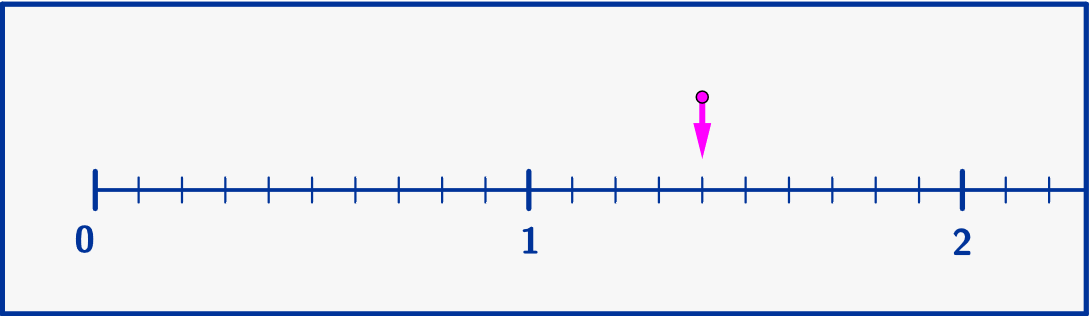
\includegraphics[width=.8\linewidth]{nombre_decimaux_demi-droite.png}
\begin{tikzpicture}[line cap=round,line join=round,>=triangle 45,x=.7cm,y=.7cm]
\clip(-7,-1.5) rectangle (11.5,2);
\fill[line width=1.2pt,color=eqeqeq,fill=eqeqeq,fill opacity=0.10000000149011612] (-6.5,2) -- (-6.5,-1.5) -- (11.,-1.5) -- (11.,2) -- cycle;
\draw[line width=1.4pt,color=qqzzff] (-3.038309699461245,4.543294499307796) -- (-1.9563840380590396,4.543294499307796);
\draw[line width=1.4pt,color=qqzzff] (-5.499690579151262,3.556818570075324) -- (-4.823487040774884,3.556818570075324);
\draw [line width=1.8pt,color=qqttzz] (-6.5,2.)-- (-6.5,-1.5);
\draw [line width=1.8pt,color=qqttzz] (-6.5,-1.5)-- (11.,-1.5);
\draw [line width=1.8pt,color=qqttzz] (11.,-1.5)-- (11.,2.);
\draw [line width=1.8pt,color=qqttzz] (11.,2.)-- (-6.5,2.);
\draw [line width=1.2pt,color=qqttzz] (-5.,-0.2)-- (-5.,0.2);
\draw [line width=1.2pt,color=qqttzz] (-4.3,-0.2)-- (-4.3,0.2);
\draw [line width=1.2pt,color=qqttzz] (-3.6,-0.2)-- (-3.6,0.2);
\draw [line width=1.2pt,color=qqttzz] (-2.9,-0.2)-- (-2.9,0.2);
\draw [line width=1.2pt,color=qqttzz] (-2.2,-0.2)-- (-2.2,0.2);
\draw [line width=1.2pt,color=qqttzz] (-1.5,-0.2)-- (-1.5,0.2);
\draw [line width=1.2pt,color=qqttzz] (-0.8,-0.2)-- (-0.8,0.2);
\draw [line width=1.2pt,color=qqttzz] (-0.1,-0.2)-- (-0.1,0.2);
\draw [line width=1.2pt,color=qqttzz] (0.6,-0.2)-- (0.6,0.2);
\draw [line width=1.2pt,color=qqttzz] (1.3,-0.2)-- (1.3,0.2);
\draw [line width=1.2pt,color=qqttzz] (2.,-0.2)-- (2.,0.2);
\draw [line width=1.2pt,color=qqttzz] (2.7,-0.2)-- (2.7,0.2);
\draw [line width=1.2pt,color=qqttzz] (3.4,-0.2)-- (3.4,0.2);
\draw [line width=1.2pt,color=qqttzz] (4.1,-0.2)-- (4.1,0.2);
\draw [line width=1.2pt,color=qqttzz] (4.8,-0.2)-- (4.8,0.2);
\draw [line width=1.2pt,color=qqttzz] (5.5,-0.2)-- (5.5,0.2);
\draw [line width=1.2pt,color=qqttzz] (6.2,-0.2)-- (6.2,0.2);
\draw [line width=1.2pt,color=qqttzz] (6.9,-0.2)-- (6.9,0.2);
\draw [line width=1.2pt,color=qqttzz] (7.6,-0.2)-- (7.6,0.2);
\draw [line width=1.2pt,color=qqttzz] (8.3,-0.2)-- (8.3,0.2);
\draw [line width=1.2pt,color=qqttzz] (9.,-0.2)-- (9.,0.2);
\draw [line width=1.2pt,color=qqttzz] (9.7,-0.2)-- (9.7,0.2);
\draw [line width=1.2pt,color=qqttzz] (10.4,-0.2)-- (10.4,0.2);
\draw [line width=1.8pt,color=qqttzz] (-5.,-0.3)-- (-5.,0.3);
\draw [line width=1.8pt,color=qqttzz] (2.,-0.3)-- (2.,0.3);
\draw [line width=1.8pt,color=qqttzz] (9.,-0.3)-- (9.,0.3);
\draw [->,line width=3.2pt,color=ffqqff] (4.8,1.5) -- (4.8,0.5);
\draw [line width=1.pt,color=qqttzz] (-5.,0.)-- (11.,0.);
\draw (1.1000559554021905,-4.680903000943034) node[anchor=north west] {0};
\draw [color=qqttzz](-5.702551640664176,-0.24500778919399624) node[anchor=north west] {$\mathbf{0}$};
\draw [color=qqttzz](1.6680669276383482,-0.29910407226410646) node[anchor=north west] {$\mathbf{1}$};
\draw [color=qqttzz](8.646487443682572,-0.2585318599615238) node[anchor=north west] {$\mathbf{2}$};
\draw [color=qqzzff](4.4,-0.2585318599615238) node[anchor=north west] {$M$};
\end{tikzpicture}
 
\end{Rep}



\begin{Rep}
L'unité est partagée en 10 parties égales, une graduation correspond à un dixième. Le point \textcolor{sacado_blue}{bleu} correspond au nombre $\textcolor{sacado_blue}{4,4}$.

Un dixième est partagé en 10 parties égales, une graduation correspond à un centième. Le point \textcolor{magenta}{violet} correspond au nombre $\textcolor{magenta}{4,46}$.

Un centième est partagé en 10 parties égales, une graduation correspond à un millième. Le point \textcolor{sacado_green}{vert} correspond au nombre $\textcolor{sacado_green}{4,465}$.


\begin{tikzpicture}[line cap=round,line join=round,>=triangle 45,x=.44cm,y=.44cm]
\clip(-5.5,-9.5) rectangle (23.5,3.5);
\fill[line width=1.2pt,color=eqeqeq,fill=eqeqeq,fill opacity=0.10000000149011612] (-5.,3.) -- (25.,3.) -- (25.,-9.) -- (-5.,-9.) -- cycle;
\draw[line width=1.4pt,color=qqzzff] (9.257484929398895,7.48867570646597) -- (13.550145734365884,7.48867570646597);
\draw [line width=1.pt,color=ffqqff] (6.,-7.)-- (16.,-7.);
\draw [line width=1.2pt,color=qqttzz] (10.5,-1.25)-- (13.5,-1.25);
\draw [line width=1.4pt,color=qqttzz] (5.,0.)-- (5.,0.75);
\draw [line width=1.4pt,color=qqttzz] (15.,0.)-- (15.,0.75);
\draw [line width=1.pt,color=qqttzz] (-5.,3.)-- (23.,3.);
\draw [line width=1.pt,color=qqttzz] (23.,3.)-- (23.,-9.);
\draw [line width=1.pt,color=qqttzz] (23.,-9.)-- (-5.,-9.);
\draw [line width=1.pt,color=qqttzz] (-5.,-9.)-- (-5.,3.);
\draw [line width=1.2pt,color=qqttzz] (4.,-1.75)-- (4.5,-1.25);
\draw [line width=1.2pt,color=qqttzz] (4.5,-1.25)-- (8.5,-1.25);
\draw [line width=1.2pt,color=qqttzz] (13.5,-1.25)-- (14.,-1.75);
\draw [line width=1.pt,color=qqzzff] (4.,-3.25)-- (14.,-3.25);
\draw [line width=1.6pt,color=qqzzff] (4.,-2.95)-- (4.,-3.55);
\draw [line width=1.6pt,color=qqzzff] (5.,-2.95)-- (5.,-3.55);
\draw [line width=1.6pt,color=qqzzff] (6.,-2.95)-- (6.,-3.55);
\draw [line width=1.6pt,color=qqzzff] (7.,-2.95)-- (7.,-3.55);
\draw [line width=1.6pt,color=qqzzff] (8.,-2.95)-- (8.,-3.55);
\draw [line width=1.6pt,color=qqzzff] (9.,-2.95)-- (9.,-3.55);
\draw [line width=1.6pt,color=qqzzff] (10.,-2.95)-- (10.,-3.55);
\draw [line width=1.6pt,color=qqzzff] (11.,-2.95)-- (11.,-3.55);
\draw [line width=1.6pt,color=qqzzff] (12.,-2.95)-- (12.,-3.55);
\draw [line width=1.6pt,color=qqzzff] (13.,-2.95)-- (13.,-3.55);
\draw [line width=1.6pt,color=qqzzff] (14.,-2.95)-- (14.,-3.55);
\draw [line width=1.2pt,color=qqttzz] (6.,-5.5)-- (6.5,-5.);
\draw [line width=1.2pt,color=qqttzz] (6.5,-5.)-- (9.5,-5.);
\draw [line width=1.2pt,color=qqttzz] (11.5,-5.)-- (15.5,-5.);
\draw [line width=1.2pt,color=qqttzz] (15.5,-5.)-- (16.,-5.5);
\draw [line width=1.pt,color=ffqqff] (6.,-6.7)-- (6.,-7.3);
\draw [line width=1.pt,color=ffqqff] (7.,-6.7)-- (7.,-7.3);
\draw [line width=1.pt,color=ffqqff] (8.,-6.7)-- (8.,-7.3);
\draw [line width=1.pt,color=ffqqff] (9.,-6.7)-- (9.,-7.3);
\draw [line width=1.pt,color=ffqqff] (10.,-6.7)-- (10.,-7.3);
\draw [line width=1.pt,color=ffqqff] (11.,-6.7)-- (11.,-7.3);
\draw [line width=1.pt,color=ffqqff] (12.,-6.7)-- (12.,-7.3);
\draw [line width=1.pt,color=ffqqff] (13.,-6.7)-- (13.,-7.3);
\draw [line width=1.pt,color=ffqqff] (14.,-6.7)-- (14.,-7.3);
\draw [line width=1.pt,color=ffqqff] (15.,-6.7)-- (15.,-7.3);
\draw [line width=1.pt,color=ffqqff] (16.,-6.7)-- (16.,-7.3);
\draw [line width=4.4pt,color=qqzzff] (9.,0.)-- (10.,0.);
\draw [line width=1.2pt,color=qqttzz] (9.5,-5.)-- (10.,-3.75);
\draw [line width=1.2pt,color=qqttzz] (11.,-3.75)-- (11.5,-5.);
\draw [line width=3.6pt,color=ffqqff] (10.,-3.25)-- (11.,-3.25);
\draw [line width=1.2pt,color=qqttzz] (10.,-0.5)-- (10.5,-1.25);
\draw [line width=1.2pt,color=qqttzz] (8.5,-1.25)-- (9.,-0.5);
\draw [line width=1.pt,color=qqzzff] (10.,0.5)-- (10.,-0.2);
\draw [line width=1.pt,color=qqzzff] (9.,0.5)-- (9.,-0.2);
\draw [line width=1.pt,color=ffqqff] (10.,-2.75)-- (10.,-3.45);
\draw [line width=1.pt,color=ffqqff] (11.,-2.75)-- (11.,-3.45);
\draw [->,line width=3.6pt,color=qqccqq] (11.,-8.5) -- (11.,-7.5);
\draw [line width=1.pt,color=qqttzz] (4.,-2.75)-- (4.,-3.75);
\draw [line width=1.pt,color=qqttzz] (14.,-2.75)-- (14.,-3.75);
\draw [line width=1.pt,color=qqttzz] (6.,-6.5)-- (6.,-7.5);
\draw [line width=1.pt,color=qqttzz] (16.,-6.5)-- (16.,-7.5);
\draw [line width=1.pt,color=qqttzz] (-5.,0.)-- (23.,0.);
\draw [color=qqttzz](4.192145179537847,2.7238222129526095) node[anchor=north west] {$\mathbf{\;8}$};
\draw [color=qqttzz](14.236971463160604,2.5950423888036) node[anchor=north west] {$\mathbf{\;9}$};
\draw [line width=1.6pt,color=qqwwzz] (-3.,-0.3)-- (-3.,0.3);
\draw [line width=1.6pt,color=qqwwzz] (-2.,-0.3)-- (-2.,0.3);
\draw [line width=1.6pt,color=qqwwzz] (-1.,-0.3)-- (-1.,0.3);
\draw [line width=1.6pt,color=qqwwzz] (0.,-0.3)-- (0.,0.3);
\draw [line width=1.6pt,color=qqwwzz] (1.,-0.3)-- (1.,0.3);
\draw [line width=1.6pt,color=qqwwzz] (2.,-0.3)-- (2.,0.3);
\draw [line width=1.6pt,color=qqwwzz] (3.,-0.3)-- (3.,0.3);
\draw [line width=1.6pt,color=qqwwzz] (4.,-0.3)-- (4.,0.3);
\draw [line width=1.6pt,color=qqwwzz] (5.,-0.3)-- (5.,0.3);
\draw [line width=1.6pt,color=qqwwzz] (6.,-0.3)-- (6.,0.3);
\draw [line width=1.6pt,color=qqwwzz] (7.,-0.3)-- (7.,0.3);
\draw [line width=1.6pt,color=qqwwzz] (8.,-0.3)-- (8.,0.3);
\draw [line width=1.6pt,color=qqwwzz] (9.,-0.3)-- (9.,0.3);
\draw [line width=1.6pt,color=qqwwzz] (10.,-0.3)-- (10.,0.3);
\draw [line width=1.6pt,color=qqwwzz] (11.,-0.3)-- (11.,0.3);
\draw [line width=1.6pt,color=qqwwzz] (12.,-0.3)-- (12.,0.3);
\draw [line width=1.6pt,color=qqwwzz] (13.,-0.3)-- (13.,0.3);
\draw [line width=1.6pt,color=qqwwzz] (14.,-0.3)-- (14.,0.3);
\draw [line width=1.6pt,color=qqwwzz] (15.,-0.3)-- (15.,0.3);
\draw [line width=1.6pt,color=qqwwzz] (16.,-0.3)-- (16.,0.3);
\draw [line width=1.6pt,color=qqwwzz] (17.,-0.3)-- (17.,0.3);
\draw [line width=1.6pt,color=qqwwzz] (18.,-0.3)-- (18.,0.3);
\draw [line width=1.6pt,color=qqwwzz] (19.,-0.3)-- (19.,0.3);
\draw [line width=1.6pt,color=qqwwzz] (20.,-0.3)-- (20.,0.3);
\draw [line width=1.6pt,color=qqwwzz] (21.,-0.3)-- (21.,0.3);
\draw [line width=1.6pt,color=qqwwzz] (22.,-0.3)-- (22.,0.3);
\draw [line width=1.8pt,color=qqttzz] (-4.,-0.3)-- (-4.,0.3);
\draw [line width=1.8pt,color=qqttzz] (0.,-0.4)-- (0.,0.5);
\draw [line width=1.8pt,color=qqttzz] (5.,-0.4)-- (5.,0.5);
\draw [line width=1.8pt,color=qqttzz] (10.,-0.4)-- (10.,0.5);
\draw [line width=1.8pt,color=qqttzz] (15.,-0.4)-- (15.,0.5);
\draw [line width=1.8pt,color=qqttzz] (20.,-0.4)-- (20.,0.5);
\draw [color=qqttzz](13.507219126316215,-1.3542055517660323) node[anchor=north west] {$\mathbf{8,5}$};
\draw [color=qqttzz](4.921897516382235,-5.174673668186655) node[anchor=north west] {$\mathbf{8,46}$};
\draw [color=qqttzz](15.138430232203671,-5.174673668186655) node[anchor=north west] {$\mathbf{8,47}$};
\draw [color=qqttzz](3.0760533702464294,-1.440058767865372) node[anchor=north west] {$\mathbf{8,4}$};
\begin{scriptsize}
\draw [fill=qqzzff] (9.,0.) circle (2.0pt);
\draw [fill=ffqqff] (10.,-3.25) circle (2.0pt);
\draw [fill=qqzzff] (9.944310658193613,7.48867570646597) circle (2.0pt);
\draw [fill=qqccqq] (11.,-7.) circle (2.0pt);
\end{scriptsize}
\end{tikzpicture}

\end{Rep}

 \end{pageCours}
 
\begin{pageAD} 

\Sf{Repérer un nombre décimal sur la droite graduée.}

\ExoCad{Représenter.}

Quelle est le nombre représenté par la flèche ? $\ldots\ldots$

 %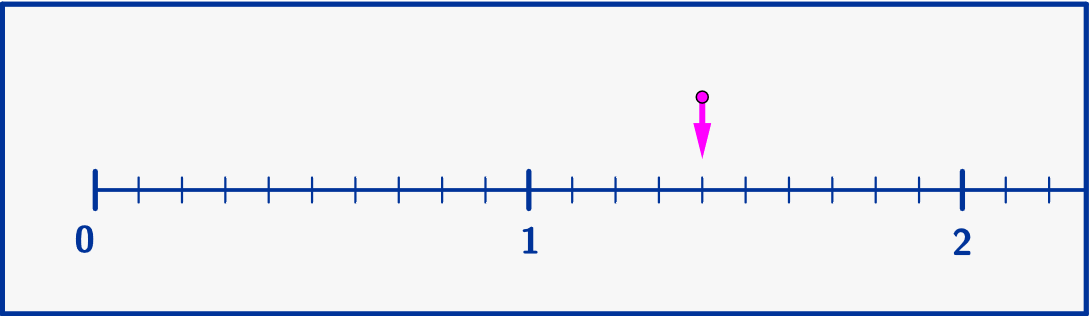
\includegraphics[width=.8\linewidth]{nombre_decimaux_demi-droite.png}
\begin{tikzpicture}[line cap=round,line join=round,>=triangle 45,x=.7cm,y=.7cm]
\clip(-7,-1.) rectangle (11.5,1.25);
\draw [line width=1.2pt,color=qqttzz] (-5.,-0.2)-- (-5.,0.2);
\draw [line width=1.2pt,color=qqttzz] (-4.3,-0.2)-- (-4.3,0.2);
\draw [line width=1.2pt,color=qqttzz] (-3.6,-0.2)-- (-3.6,0.2);
\draw [line width=1.2pt,color=qqttzz] (-2.9,-0.2)-- (-2.9,0.2);
\draw [line width=1.2pt,color=qqttzz] (-2.2,-0.2)-- (-2.2,0.2);
\draw [line width=1.2pt,color=qqttzz] (-1.5,-0.2)-- (-1.5,0.2);
\draw [line width=1.2pt,color=qqttzz] (-0.8,-0.2)-- (-0.8,0.2);
\draw [line width=1.2pt,color=qqttzz] (-0.1,-0.2)-- (-0.1,0.2);
\draw [line width=1.2pt,color=qqttzz] (0.6,-0.2)-- (0.6,0.2);
\draw [line width=1.2pt,color=qqttzz] (1.3,-0.2)-- (1.3,0.2);
\draw [line width=1.2pt,color=qqttzz] (2.,-0.2)-- (2.,0.2);
\draw [line width=1.2pt,color=qqttzz] (2.7,-0.2)-- (2.7,0.2);
\draw [line width=1.2pt,color=qqttzz] (3.4,-0.2)-- (3.4,0.2);
\draw [line width=1.2pt,color=qqttzz] (4.1,-0.2)-- (4.1,0.2);
\draw [line width=1.2pt,color=qqttzz] (4.8,-0.2)-- (4.8,0.2);
\draw [line width=1.2pt,color=qqttzz] (5.5,-0.2)-- (5.5,0.2);
\draw [line width=1.2pt,color=qqttzz] (6.2,-0.2)-- (6.2,0.2);
\draw [line width=1.2pt,color=qqttzz] (6.9,-0.2)-- (6.9,0.2);
\draw [line width=1.2pt,color=qqttzz] (7.6,-0.2)-- (7.6,0.2);
\draw [line width=1.2pt,color=qqttzz] (8.3,-0.2)-- (8.3,0.2);
\draw [line width=1.2pt,color=qqttzz] (9.,-0.2)-- (9.,0.2);
\draw [line width=1.2pt,color=qqttzz] (9.7,-0.2)-- (9.7,0.2);
\draw [line width=1.2pt,color=qqttzz] (10.4,-0.2)-- (10.4,0.2);
\draw [line width=1.8pt,color=qqttzz] (-5.,-0.3)-- (-5.,0.3);
\draw [line width=1.8pt,color=qqttzz] (2.,-0.3)-- (2.,0.3);
\draw [line width=1.8pt,color=qqttzz] (9.,-0.3)-- (9.,0.3);
\draw [->,line width=3.2pt,color=ffqqff] (0.65,1.5) -- (0.65,0.5);
\draw [line width=1.pt,color=qqttzz] (-5.1,0.)-- (11.,0.);
\draw [color=qqttzz](-5.702551640664176,-0.24500778919399624) node[anchor=north west] {$\mathbf{4}$};
\draw [color=qqttzz](1.6680669276383482,-0.29910407226410646) node[anchor=north west] {$\mathbf{5}$};
\draw [color=qqttzz](8.646487443682572,-0.2585318599615238) node[anchor=north west] {$\mathbf{6}$};
\end{tikzpicture}
 


\ExoCad{Représenter.}

On a placé 3 points sur la droite graduée.

\begin{tikzpicture}[line cap=round,line join=round,>=triangle 45,x=.7cm,y=.7cm]
\clip(-7,-1.) rectangle (11.5,1.25);
\draw [line width=1.2pt,color=qqttzz] (-5.,-0.2)-- (-5.,0.2);
\draw [line width=1.2pt,color=qqttzz] (-4.3,-0.2)-- (-4.3,0.2);
\draw [line width=1.2pt,color=qqttzz] (-3.6,-0.2)-- (-3.6,0.2);
\draw [line width=1.2pt,color=qqttzz] (-2.9,-0.2)-- (-2.9,0.2);
\draw [line width=1.2pt,color=qqttzz] (-2.2,-0.2)-- (-2.2,0.2);
\draw [line width=1.2pt,color=qqttzz] (-1.5,-0.2)-- (-1.5,0.2);
\draw [line width=1.2pt,color=qqttzz] (-0.8,-0.2)-- (-0.8,0.2);
\draw [line width=1.2pt,color=qqttzz] (-0.1,-0.2)-- (-0.1,0.2);
\draw [line width=1.2pt,color=qqttzz] (0.6,-0.2)-- (0.6,0.2);
\draw [line width=1.2pt,color=qqttzz] (1.3,-0.2)-- (1.3,0.2);
\draw [line width=1.2pt,color=qqttzz] (2.,-0.2)-- (2.,0.2);
\draw [line width=1.2pt,color=qqttzz] (2.7,-0.2)-- (2.7,0.2);
\draw [line width=1.2pt,color=qqttzz] (3.4,-0.2)-- (3.4,0.2);
\draw [line width=1.2pt,color=qqttzz] (4.1,-0.2)-- (4.1,0.2);
\draw [line width=1.2pt,color=qqttzz] (4.8,-0.2)-- (4.8,0.2);
\draw [line width=1.2pt,color=qqttzz] (5.5,-0.2)-- (5.5,0.2);
\draw [line width=1.2pt,color=qqttzz] (6.2,-0.2)-- (6.2,0.2);
\draw [line width=1.2pt,color=qqttzz] (6.9,-0.2)-- (6.9,0.2);
\draw [line width=1.2pt,color=qqttzz] (7.6,-0.2)-- (7.6,0.2);
\draw [line width=1.2pt,color=qqttzz] (8.3,-0.2)-- (8.3,0.2);
\draw [line width=1.2pt,color=qqttzz] (9.,-0.2)-- (9.,0.2);
\draw [line width=1.2pt,color=qqttzz] (9.7,-0.2)-- (9.7,0.2);
\draw [line width=1.2pt,color=qqttzz] (10.4,-0.2)-- (10.4,0.2);
\draw [line width=1.8pt,color=qqttzz] (-5.,-0.3)-- (-5.,0.3);
\draw [line width=1.8pt,color=qqttzz] (2.,-0.3)-- (2.,0.3);
\draw [line width=1.8pt,color=qqttzz] (9.,-0.3)-- (9.,0.3);
\draw [line width=1.pt,color=qqttzz] (-5.5,0.)-- (11.,0.);
\draw [color=qqttzz](-5.702551640664176,-0.24500778919399624) node[anchor=north west] {$\mathbf{12}$};
\draw [color=qqttzz](1.6680669276383482,-0.29910407226410646) node[anchor=north west] {$\mathbf{13}$};
\draw [color=qqttzz](8.646487443682572,-0.2585318599615238) node[anchor=north west] {$\mathbf{14}$};
\draw [color=qqttzz](9.95,0.8585318599615238) node[anchor=north west] {$C$};
\draw [color=qqttzz](4.35,0.8585318599615238) node[anchor=north west] {$A$};
\draw [color=qqttzz](-2.05,0.8585318599615238) node[anchor=north west] {$B$};
\end{tikzpicture}

\begin{enumerate}
\item Quelle est l'abscisse du point A ? $\ldots\ldots$
\item Quelle est l'abscisse du point B ? $\ldots\ldots$ 
\item Quelle est l'abscisse du point C ? $\ldots\ldots$
\end{enumerate}



\ExoCad{Représenter.}

On a tracé la droite graduée.

\begin{tikzpicture}[line cap=round,line join=round,>=triangle 45,x=.7cm,y=.7cm]
\clip(-7,-1.) rectangle (11.5,1);
\draw [line width=1.2pt,color=qqttzz] (-5.,-0.2)-- (-5.,0.2);
\draw [line width=1.2pt,color=qqttzz] (-4.3,-0.2)-- (-4.3,0.2);
\draw [line width=1.2pt,color=qqttzz] (-3.6,-0.2)-- (-3.6,0.2);
\draw [line width=1.2pt,color=qqttzz] (-2.9,-0.2)-- (-2.9,0.2);
\draw [line width=1.2pt,color=qqttzz] (-2.2,-0.2)-- (-2.2,0.2);
\draw [line width=1.2pt,color=qqttzz] (-1.5,-0.2)-- (-1.5,0.2);
\draw [line width=1.2pt,color=qqttzz] (-0.8,-0.2)-- (-0.8,0.2);
\draw [line width=1.2pt,color=qqttzz] (-0.1,-0.2)-- (-0.1,0.2);
\draw [line width=1.2pt,color=qqttzz] (0.6,-0.2)-- (0.6,0.2);
\draw [line width=1.2pt,color=qqttzz] (1.3,-0.2)-- (1.3,0.2);
\draw [line width=1.2pt,color=qqttzz] (2.,-0.2)-- (2.,0.2);
\draw [line width=1.2pt,color=qqttzz] (2.7,-0.2)-- (2.7,0.2);
\draw [line width=1.2pt,color=qqttzz] (3.4,-0.2)-- (3.4,0.2);
\draw [line width=1.2pt,color=qqttzz] (4.1,-0.2)-- (4.1,0.2);
\draw [line width=1.2pt,color=qqttzz] (4.8,-0.2)-- (4.8,0.2);
\draw [line width=1.2pt,color=qqttzz] (5.5,-0.2)-- (5.5,0.2);
\draw [line width=1.2pt,color=qqttzz] (6.2,-0.2)-- (6.2,0.2);
\draw [line width=1.2pt,color=qqttzz] (6.9,-0.2)-- (6.9,0.2);
\draw [line width=1.2pt,color=qqttzz] (7.6,-0.2)-- (7.6,0.2);
\draw [line width=1.2pt,color=qqttzz] (8.3,-0.2)-- (8.3,0.2);
\draw [line width=1.2pt,color=qqttzz] (9.,-0.2)-- (9.,0.2);
\draw [line width=1.2pt,color=qqttzz] (9.7,-0.2)-- (9.7,0.2);
\draw [line width=1.2pt,color=qqttzz] (10.4,-0.2)-- (10.4,0.2);
\draw [line width=1.8pt,color=qqttzz] (-5.,-0.3)-- (-5.,0.3);
\draw [line width=1.8pt,color=qqttzz] (2.,-0.3)-- (2.,0.3);
\draw [line width=1.8pt,color=qqttzz] (9.,-0.3)-- (9.,0.3);
\draw [line width=1.pt,color=qqttzz] (-5.1,0.)-- (11.,0.);
\draw [color=qqttzz](-5.702551640664176,-0.24500778919399624) node[anchor=north west] {$\mathbf{8,5}$};
\draw [color=qqttzz](1.6680669276383482,-0.29910407226410646) node[anchor=north west] {$\mathbf{8,6}$};
\draw [color=qqttzz](8.646487443682572,-0.2585318599615238) node[anchor=north west] {$\mathbf{8,7}$};
\end{tikzpicture}

\begin{enumerate}
\item Place le nombre $8,62$.
\item Place le point $M$ d'abscisse le nombre $8,58$.
\end{enumerate}


\ExoCad{Représenter.}

Quelle est le nombre représenté par la flèche ? $\ldots\ldots$

\begin{tikzpicture}[line cap=round,line join=round,>=triangle 45,x=.44cm,y=.44cm]
\clip(-5.5,-9.5) rectangle (23.5,3.5);
\fill[line width=1.2pt,color=eqeqeq,fill=eqeqeq,fill opacity=0.10000000149011612] (-5.,3.) -- (25.,3.) -- (25.,-9.) -- (-5.,-9.) -- cycle;
\draw[line width=1.4pt,color=qqzzff] (9.257484929398895,7.48867570646597) -- (13.550145734365884,7.48867570646597);
\draw [line width=1.pt,color=ffqqff] (6.,-7.)-- (16.,-7.);
\draw [line width=1.2pt,color=qqttzz] (10.5,-1.25)-- (13.5,-1.25);
\draw [line width=1.4pt,color=qqttzz] (5.,0.)-- (5.,0.75);
\draw [line width=1.4pt,color=qqttzz] (15.,0.)-- (15.,0.75);
\draw [line width=1.pt,color=qqttzz] (-5.,3.)-- (23.,3.);
\draw [line width=1.pt,color=qqttzz] (23.,3.)-- (23.,-9.);
\draw [line width=1.pt,color=qqttzz] (23.,-9.)-- (-5.,-9.);
\draw [line width=1.pt,color=qqttzz] (-5.,-9.)-- (-5.,3.);
\draw [line width=1.2pt,color=qqttzz] (4.,-1.75)-- (4.5,-1.25);
\draw [line width=1.2pt,color=qqttzz] (4.5,-1.25)-- (8.5,-1.25);
\draw [line width=1.2pt,color=qqttzz] (13.5,-1.25)-- (14.,-1.75);
\draw [line width=1.pt,color=qqzzff] (4.,-3.25)-- (14.,-3.25);
\draw [line width=1.6pt,color=qqzzff] (4.,-2.95)-- (4.,-3.55);
\draw [line width=1.6pt,color=qqzzff] (5.,-2.95)-- (5.,-3.55);
\draw [line width=1.6pt,color=qqzzff] (6.,-2.95)-- (6.,-3.55);
\draw [line width=1.6pt,color=qqzzff] (7.,-2.95)-- (7.,-3.55);
\draw [line width=1.6pt,color=qqzzff] (8.,-2.95)-- (8.,-3.55);
\draw [line width=1.6pt,color=qqzzff] (9.,-2.95)-- (9.,-3.55);
\draw [line width=1.6pt,color=qqzzff] (10.,-2.95)-- (10.,-3.55);
\draw [line width=1.6pt,color=qqzzff] (11.,-2.95)-- (11.,-3.55);
\draw [line width=1.6pt,color=qqzzff] (12.,-2.95)-- (12.,-3.55);
\draw [line width=1.6pt,color=qqzzff] (13.,-2.95)-- (13.,-3.55);
\draw [line width=1.6pt,color=qqzzff] (14.,-2.95)-- (14.,-3.55);
\draw [line width=1.2pt,color=qqttzz] (6.,-5.5)-- (6.5,-5.);
\draw [line width=1.2pt,color=qqttzz] (6.5,-5.)-- (9.5,-5.);
\draw [line width=1.2pt,color=qqttzz] (11.5,-5.)-- (15.5,-5.);
\draw [line width=1.2pt,color=qqttzz] (15.5,-5.)-- (16.,-5.5);
\draw [line width=1.pt,color=ffqqff] (6.,-6.7)-- (6.,-7.3);
\draw [line width=1.pt,color=ffqqff] (7.,-6.7)-- (7.,-7.3);
\draw [line width=1.pt,color=ffqqff] (8.,-6.7)-- (8.,-7.3);
\draw [line width=1.pt,color=ffqqff] (9.,-6.7)-- (9.,-7.3);
\draw [line width=1.pt,color=ffqqff] (10.,-6.7)-- (10.,-7.3);
\draw [line width=1.pt,color=ffqqff] (11.,-6.7)-- (11.,-7.3);
\draw [line width=1.pt,color=ffqqff] (12.,-6.7)-- (12.,-7.3);
\draw [line width=1.pt,color=ffqqff] (13.,-6.7)-- (13.,-7.3);
\draw [line width=1.pt,color=ffqqff] (14.,-6.7)-- (14.,-7.3);
\draw [line width=1.pt,color=ffqqff] (15.,-6.7)-- (15.,-7.3);
\draw [line width=1.pt,color=ffqqff] (16.,-6.7)-- (16.,-7.3);
\draw [line width=4.4pt,color=qqzzff] (9.,0.)-- (10.,0.);
\draw [line width=1.2pt,color=qqttzz] (9.5,-5.)-- (10.,-3.75);
\draw [line width=1.2pt,color=qqttzz] (11.,-3.75)-- (11.5,-5.);
\draw [line width=3.6pt,color=ffqqff] (10.,-3.25)-- (11.,-3.25);
\draw [line width=1.2pt,color=qqttzz] (10.,-0.5)-- (10.5,-1.25);
\draw [line width=1.2pt,color=qqttzz] (8.5,-1.25)-- (9.,-0.5);
\draw [line width=1.pt,color=qqzzff] (10.,0.5)-- (10.,-0.2);
\draw [line width=1.pt,color=qqzzff] (9.,0.5)-- (9.,-0.2);
\draw [line width=1.pt,color=ffqqff] (10.,-2.75)-- (10.,-3.45);
\draw [line width=1.pt,color=ffqqff] (11.,-2.75)-- (11.,-3.45);
\draw [line width=1.pt,color=qqttzz] (4.,-2.75)-- (4.,-3.75);
\draw [line width=1.pt,color=qqttzz] (14.,-2.75)-- (14.,-3.75);
\draw [line width=1.pt,color=qqttzz] (6.,-6.5)-- (6.,-7.5);
\draw [line width=1.pt,color=qqttzz] (16.,-6.5)-- (16.,-7.5);
\draw [line width=1.pt,color=qqttzz] (-5.,0.)-- (23.,0.);
\draw [color=qqttzz](4.192145179537847,2.7238222129526095) node[anchor=north west] {$\mathbf{\;6}$};
\draw [color=qqttzz](14.236971463160604,2.5950423888036) node[anchor=north west] {$\mathbf{\;7}$};
\draw [line width=1.6pt,color=qqwwzz] (-3.,-0.3)-- (-3.,0.3);
\draw [line width=1.6pt,color=qqwwzz] (-2.,-0.3)-- (-2.,0.3);
\draw [line width=1.6pt,color=qqwwzz] (-1.,-0.3)-- (-1.,0.3);
\draw [line width=1.6pt,color=qqwwzz] (0.,-0.3)-- (0.,0.3);
\draw [line width=1.6pt,color=qqwwzz] (1.,-0.3)-- (1.,0.3);
\draw [line width=1.6pt,color=qqwwzz] (2.,-0.3)-- (2.,0.3);
\draw [line width=1.6pt,color=qqwwzz] (3.,-0.3)-- (3.,0.3);
\draw [line width=1.6pt,color=qqwwzz] (4.,-0.3)-- (4.,0.3);
\draw [line width=1.6pt,color=qqwwzz] (5.,-0.3)-- (5.,0.3);
\draw [line width=1.6pt,color=qqwwzz] (6.,-0.3)-- (6.,0.3);
\draw [line width=1.6pt,color=qqwwzz] (7.,-0.3)-- (7.,0.3);
\draw [line width=1.6pt,color=qqwwzz] (8.,-0.3)-- (8.,0.3);
\draw [line width=1.6pt,color=qqwwzz] (9.,-0.3)-- (9.,0.3);
\draw [line width=1.6pt,color=qqwwzz] (10.,-0.3)-- (10.,0.3);
\draw [line width=1.6pt,color=qqwwzz] (11.,-0.3)-- (11.,0.3);
\draw [line width=1.6pt,color=qqwwzz] (12.,-0.3)-- (12.,0.3);
\draw [line width=1.6pt,color=qqwwzz] (13.,-0.3)-- (13.,0.3);
\draw [line width=1.6pt,color=qqwwzz] (14.,-0.3)-- (14.,0.3);
\draw [line width=1.6pt,color=qqwwzz] (15.,-0.3)-- (15.,0.3);
\draw [line width=1.6pt,color=qqwwzz] (16.,-0.3)-- (16.,0.3);
\draw [line width=1.6pt,color=qqwwzz] (17.,-0.3)-- (17.,0.3);
\draw [line width=1.6pt,color=qqwwzz] (18.,-0.3)-- (18.,0.3);
\draw [line width=1.6pt,color=qqwwzz] (19.,-0.3)-- (19.,0.3);
\draw [line width=1.6pt,color=qqwwzz] (20.,-0.3)-- (20.,0.3);
\draw [line width=1.6pt,color=qqwwzz] (21.,-0.3)-- (21.,0.3);
\draw [line width=1.6pt,color=qqwwzz] (22.,-0.3)-- (22.,0.3);
\draw [line width=1.8pt,color=qqttzz] (-4.,-0.3)-- (-4.,0.3);
\draw [line width=1.8pt,color=qqttzz] (0.,-0.4)-- (0.,0.5);
\draw [line width=1.8pt,color=qqttzz] (5.,-0.4)-- (5.,0.5);
\draw [line width=1.8pt,color=qqttzz] (10.,-0.4)-- (10.,0.5);
\draw [line width=1.8pt,color=qqttzz] (15.,-0.4)-- (15.,0.5);
\draw [line width=1.8pt,color=qqttzz] (20.,-0.4)-- (20.,0.5);
\draw [->,line width=3.6pt,color=qqccqq] (9.,-8.5) -- (9.,-7.5);
\begin{scriptsize}
\draw [fill=qqzzff] (9.,0.) circle (2.0pt);
\draw [fill=ffqqff] (10.,-3.25) circle (2.0pt);
\draw [fill=qqzzff] (9.944310658193613,7.48867570646597) circle (2.0pt);
\draw [fill=qqccqq] (9.,-7.) circle (2.0pt);
\end{scriptsize}
\end{tikzpicture}

\end{pageAD}


\begin{pageCours}

\section{Encadrer un nombre décimal}

\begin{Def}
\textbf{Encadrer} un nombre, c'est trouver un nombre plus petit et un nombre plus grand. La \textbf{précision de l'encadrement} est la \textbf{différence} entre les deux nombres trouvés.
\end{Def}

\begin{Ex}
Encadrement du nombre $5,65$ :
 \begin{itemize}[leftmargin=*]
\item Encadrement à l'unité : \(5,0 < 5,65< 6,0\)

\item Encadrement au dixième : \(5,6 < 5,65< 5,7\)
 \end{itemize}
\end{Ex}


\begin{DefT}{Valeur par défaut.  Valeur par excès}
Dans l'encadrement  : \(5,0 < 5,65 < 6,0\), le nombre inférieur de l'encadrement est appelé la \textbf{valeur par défaut}\index{valeur par défaut} de $5,65$ et le nombre supérieur de l'encadrement est appelé la \textbf{valeur par excès}\index{valeur par excès} de $5,65$.
\end{DefT}



\section{Ranger, classer des nombres décimaux}

\begin{DefT}{Ordre croissant. Ordre décroissant}
\begin{itemize}[leftmargin=*]
\item Ranger des nombres dans \textbf{l'ordre croissant}\index{Ordre croissant} signifie les ranger \textbf{du plus petit au plus grand}.
\item Ranger des nombres dans \textbf{l'ordre décroissant}\index{Ordre décroissant} signifie les ranger \textbf{du plus grand au plus petit}.
\end{itemize}
\end{DefT}

\end{pageCours}

\begin{pageAD} 

\Sf{Encadrer un nombre décimal avec une précision donnée.}

\ExoCad{Représenter. Communiquer.}

Lou  achete un livre à 7,30 \euro , un manga à 9,49\euro . Donne un \textbf{ordre de grandeur} du prix que Lou doit payer ?
 
\point{3}


\ExoCad{Représenter. Communiquer.}

\begin{enumerate}
\item Encadrer le nombre $33,93$ au \textbf{dixième} près.
 \point{2}
 \item Encadrer le nombre $262,679$ au \textbf{centième} près.
 \point{2}
\item Encadrer le nombre $134,15$ à l'\textbf{unité} près.
 \point{2} 
\item Encadrer le nombre $8,246$ au \textbf{millième} près.
 \point{2}  
\end{enumerate}

\Sf{Ranger, classer les nombres décimaux}


\ExoCad{Représenter. Communiquer.}

Complète 
\begin{enumerate}
\item au \textbf{dixième} près : $\ldots \ldots < 43,78 < \ldots \ldots $
\item au \textbf{centième} près : $\ldots \ldots < 25,067 < \ldots \ldots $
\item au \textbf{millième} près : $\ldots \ldots < 20,0023 < \ldots \ldots $
\end{enumerate}




\ExoCad{Représenter. Communiquer.}

Ranger les nombres suivants dans l'ordre croissant : \[35,73\;-\;83,8\;-\;615,8\;-\;2,704\]

\end{pageAD} 



\begin{pageParcoursu} 

\ExoCu{Modéliser. Calculer.}

Je suis un nombre décimal entre  $9,1$ et $9,2$.\vspace{0.3cm}

Je suis $\ldots \ldots\ldots$



\ExoCu{Représenter. Communiquer.}

À partir des renseignements qui suivent, trouve le nombre caché :

\begin{itemize}
\item  Je suis un nombre décimal de 3 chiffres.
\item  Son chiffre des dixièmes est le même que celui de 67,25.
\item  Son chiffre des centièmes est le chiffre des unités de milliers de 215 006.
\item  Son chiffre des unités est le double de son chiffre dixièmes.
\end{itemize}
 
Je suis : $\_\_$ $\_\_$ $\_\_$ 
 
\ExoCu{Modéliser. Calculer.}

Encadre le nombre $25,63$ :

\begin{itemize}
\item par deux nombres entiers consécutifs : $\ldots\ldots\ldots$ et $\ldots\ldots\ldots$ \vspace{0.3cm}
\item par deux nombres décimaux, au dixième près : $\ldots\ldots\ldots$ et $\ldots\ldots\ldots$ \vspace{0.3cm}
\end{itemize} 
 
 
\ExoCu{Représenter.}

Écris de différentes façons le nombre $12,06$.

\begin{itemize}
\item $2,5 = \ldots\ldots\ldots$ unités et $\ldots\ldots\ldots$ dixièmes \vspace{0.3cm}
\item $12,06 =\ldots\ldots\ldots  \ldots\ldots\ldots \ldots\ldots\ldots$ centièmes\vspace{0.3cm}
\item $25,36 =\ldots\times 10 + \ldots\times 1 + \ldots\times \dfrac{1}{10} +  \ldots\times \dfrac{1}{100}$ 
\end{itemize}

\ExoCu{Représenter.}

Donne une écriture décimale de chaque nombre. 

\begin{minipage}{0.32\linewidth}
 $\dfrac{54}{10} =  \ldots\ldots\ldots$ 
\end{minipage}
\begin{minipage}{0.32\linewidth}
$\dfrac{2341}{100} =  \ldots\ldots\ldots$  
\end{minipage}
\begin{minipage}{0.32\linewidth}
$\dfrac{5064}{1000} =  \ldots\ldots\ldots$   
\end{minipage}
 
\ExoCu{Représenter.}
 
Donne l'abscisse du point représenté en rouge :  $\ldots\ldots\ldots$
 
\definecolor{ffqqqq}{rgb}{1.,0.,0.}
\definecolor{yqyqyq}{rgb}{0.5019607843137255,0.5019607843137255,0.5019607843137255}
\begin{tikzpicture}[line cap=round,line join=round,>=triangle 45,x=1.0cm,y=1.0cm]
\clip(1.66,0.69) rectangle (13.04,2.85);
\draw [color=yqyqyq](1.82,2.71) node[anchor=north west] {$6$};
\draw [color=yqyqyq](11.8,2.73) node[anchor=north west] {$7$};
\draw [line width=1.pt,color=yqyqyq] (2.,2.)-- (12.,2.);
\draw [line width=1.pt,color=yqyqyq] (4.5,0.94)-- (8.,2.);
\draw [line width=1.pt,color=yqyqyq] (12.227272727272728,0.9945454545454545)-- (9.,2.);
\draw [line width=1.pt,color=yqyqyq] (4.5,0.94)-- (12.227272727272728,0.9945454545454545);
\begin{scriptsize}
\draw [color=yqyqyq] (2.,2.)-- ++(-2.5pt,0 pt) -- ++(5.0pt,0 pt) ++(-2.5pt,-2.5pt) -- ++(0 pt,5.0pt);
\draw [color=yqyqyq] (3.,2.)-- ++(-2.5pt,0 pt) -- ++(5.0pt,0 pt) ++(-2.5pt,-2.5pt) -- ++(0 pt,5.0pt);
\draw [color=yqyqyq] (4.,2.)-- ++(-2.5pt,0 pt) -- ++(5.0pt,0 pt) ++(-2.5pt,-2.5pt) -- ++(0 pt,5.0pt);
\draw [color=yqyqyq] (5.,2.)-- ++(-2.5pt,0 pt) -- ++(5.0pt,0 pt) ++(-2.5pt,-2.5pt) -- ++(0 pt,5.0pt);
\draw [color=yqyqyq] (6.,2.)-- ++(-2.5pt,0 pt) -- ++(5.0pt,0 pt) ++(-2.5pt,-2.5pt) -- ++(0 pt,5.0pt);
\draw [color=yqyqyq] (7.,2.)-- ++(-2.5pt,0 pt) -- ++(5.0pt,0 pt) ++(-2.5pt,-2.5pt) -- ++(0 pt,5.0pt);
\draw [color=yqyqyq] (8.,2.)-- ++(-2.5pt,0 pt) -- ++(5.0pt,0 pt) ++(-2.5pt,-2.5pt) -- ++(0 pt,5.0pt);
\draw [color=yqyqyq] (9.,2.)-- ++(-2.5pt,0 pt) -- ++(5.0pt,0 pt) ++(-2.5pt,-2.5pt) -- ++(0 pt,5.0pt);
\draw [color=yqyqyq] (10.,2.)-- ++(-2.5pt,0 pt) -- ++(5.0pt,0 pt) ++(-2.5pt,-2.5pt) -- ++(0 pt,5.0pt);
\draw [color=yqyqyq] (11.,2.)-- ++(-2.5pt,0 pt) -- ++(5.0pt,0 pt) ++(-2.5pt,-2.5pt) -- ++(0 pt,5.0pt);
\draw [color=yqyqyq] (12.,2.)-- ++(-2.5pt,0 pt) -- ++(5.0pt,0 pt) ++(-2.5pt,-2.5pt) -- ++(0 pt,5.0pt);
\draw [color=yqyqyq] (4.5,0.94)-- ++(-2.5pt,0 pt) -- ++(5.0pt,0 pt) ++(-2.5pt,-2.5pt) -- ++(0 pt,5.0pt);
\draw [color=yqyqyq] (5.2727272727272725,0.9454545454545454)-- ++(-2.5pt,0 pt) -- ++(5.0pt,0 pt) ++(-2.5pt,-2.5pt) -- ++(0 pt,5.0pt);
\draw [color=yqyqyq] (6.045454545454545,0.9509090909090908)-- ++(-2.5pt,0 pt) -- ++(5.0pt,0 pt) ++(-2.5pt,-2.5pt) -- ++(0 pt,5.0pt);
\draw [color=yqyqyq] (6.8181818181818175,0.9563636363636363)-- ++(-2.5pt,0 pt) -- ++(5.0pt,0 pt) ++(-2.5pt,-2.5pt) -- ++(0 pt,5.0pt);
\draw [color=yqyqyq] (7.590909090909091,0.9618181818181818)-- ++(-2.5pt,0 pt) -- ++(5.0pt,0 pt) ++(-2.5pt,-2.5pt) -- ++(0 pt,5.0pt);
\draw [color=yqyqyq] (8.363636363636363,0.9672727272727273)-- ++(-2.5pt,0 pt) -- ++(5.0pt,0 pt) ++(-2.5pt,-2.5pt) -- ++(0 pt,5.0pt);
\draw [color=yqyqyq] (9.136363636363637,0.9727272727272727)-- ++(-2.5pt,0 pt) -- ++(5.0pt,0 pt) ++(-2.5pt,-2.5pt) -- ++(0 pt,5.0pt);
\draw [color=yqyqyq] (9.90909090909091,0.9781818181818182)-- ++(-2.5pt,0 pt) -- ++(5.0pt,0 pt) ++(-2.5pt,-2.5pt) -- ++(0 pt,5.0pt);
\draw [color=ffqqqq] (10.699902842211321,0.9837640200626683)-- ++(-2.5pt,0 pt) -- ++(5.0pt,0 pt) ++(-2.5pt,-2.5pt) -- ++(0 pt,5.0pt);
\draw [color=yqyqyq] (11.454545454545455,0.9890909090909091)-- ++(-2.5pt,0 pt) -- ++(5.0pt,0 pt) ++(-2.5pt,-2.5pt) -- ++(0 pt,5.0pt);
\draw [color=yqyqyq] (12.227272727272728,0.9945454545454545)-- ++(-2.5pt,0 pt) -- ++(5.0pt,0 pt) ++(-2.5pt,-2.5pt) -- ++(0 pt,5.0pt);
\end{scriptsize}
\end{tikzpicture}

\end{pageParcoursu}



\begin{pageParcoursd} 

\ExoCd{Modéliser. Calculer.}

Propose un nombre décimal intercalé entre $3,451$ et $3,452$ : $\ldots \ldots\ldots \ldots$

\ExoCd{Modéliser. Calculer.}

Encadre le nombre $99,98$ :
\begin{itemize}
\item par deux nombres décimaux, au dixième près : $\ldots\ldots\ldots$ et $\ldots\ldots\ldots$ \vspace{0.3cm}
\item par deux nombres décimaux, au centièmes près : $\ldots\ldots\ldots$ et $\ldots\ldots\ldots$
\end{itemize}
 
 

\ExoCd{Représenter.}

Écris de différentes façons le nombre $42,3065$.

\begin{itemize}
\item $42,3065 = \ldots\ldots\ldots$ unités et $\ldots\ldots\ldots$ dix-millièmes   $ = \ldots\ldots\ldots \ldots\ldots\ldots$ dix-millièmes\vspace{0.3cm}
\item $42,3065 = \ldots\times 10 + \ldots\times 1 + \ldots\times \dfrac{1}{10} +  \ldots\times \dfrac{1}{100} +  \ldots\times \dfrac{1}{1000} + \ldots\times \dfrac{1}{\np{10000}}$ \vspace{0.3cm}
\end{itemize}


\ExoCd{Représenter.}

À partir des renseignements qui suivent, trouve le nombre caché :

\begin{itemize}
\item  On cherche un nombre décimal de 5 chiffres.
\item  Son chiffre des dixièmes est le même que celui de 17,54.
\item  Son chiffre des centièmes est le chiffre des unités de millions de 738 214 006.
\item  Son chiffre des unités est le chiffre des dizaines de mille de 120 008.
\item  Son chiffre des millièmes est la moitié de celui des centièmes.
\item  Son chiffre des dix-millièmes est égal au chiffre des unités.
\end{itemize}

Je suis : $\_\_$ $\_\_$ $\_\_$ $\_\_$ $\_\_$   
 

\ExoCd{Représenter.}

Entoure les nombres égaux  dans la liste proposée : 
$$\dfrac{250}{1000} \quad  \dfrac{1284}{10000} \quad \dfrac{1}{4}  \quad 0,25 \quad 1,4 \quad \dfrac{25}{100}$$
 
\ExoCd{Représenter.}
 
Donne l'abscisse du point représenté en rouge :  $\ldots\ldots\ldots$
 
\definecolor{yqyqyq}{rgb}{0.5019607843137255,0.5019607843137255,0.5019607843137255}
\definecolor{ffqqqq}{rgb}{1.,0.,0.}
\definecolor{ududff}{rgb}{0.30196078431372547,0.30196078431372547,1.}
\begin{tikzpicture}[line cap=round,line join=round,>=triangle 45,x=1.0cm,y=1.0cm]
\clip(1.26,-0.37) rectangle (13.56,3.01);
\draw [color=ududff](1.56,2.57) node[anchor=north west] {$164$};
\draw [color=ududff](11.56,2.57) node[anchor=north west] {$165$};
\draw [line width=1.pt,color=ududff] (2.,2.)-- (12.,2.);
\draw [line width=1.pt,color=yqyqyq] (4.5,0.94)-- (8.,2.);
\draw [line width=1.pt,color=yqyqyq] (12.227272727272728,0.9945454545454545)-- (9.,2.);
\draw [line width=1.pt,color=yqyqyq] (6.4,0.)-- (9.136363636363637,0.9727272727272727);
\draw [line width=1.pt,color=yqyqyq] (12.4,0.)-- (9.90909090909091,0.9781818181818182);
\draw [line width=1.pt,color=ududff] (4.5,0.94)-- (12.227272727272728,0.9945454545454545);
\draw [line width=1.pt,color=ududff] (6.4,0.)-- (12.4,0.);
\begin{scriptsize}
\draw [color=ududff] (6.4,0.)-- ++(-2.5pt,0 pt) -- ++(5.0pt,0 pt) ++(-2.5pt,-2.5pt) -- ++(0 pt,5.0pt);
\draw [color=ududff] (7.,0.)-- ++(-2.5pt,0 pt) -- ++(5.0pt,0 pt) ++(-2.5pt,-2.5pt) -- ++(0 pt,5.0pt);
\draw [color=ududff] (7.6,0.)-- ++(-2.5pt,0 pt) -- ++(5.0pt,0 pt) ++(-2.5pt,-2.5pt) -- ++(0 pt,5.0pt);
\draw [color=ududff] (8.2,0.)-- ++(-2.5pt,0 pt) -- ++(5.0pt,0 pt) ++(-2.5pt,-2.5pt) -- ++(0 pt,5.0pt);
\draw [color=ffqqqq] (8.8,0.)-- ++(-2.5pt,0 pt) -- ++(5.0pt,0 pt) ++(-2.5pt,-2.5pt) -- ++(0 pt,5.0pt);
\draw [color=ududff] (9.4,0.)-- ++(-2.5pt,0 pt) -- ++(5.0pt,0 pt) ++(-2.5pt,-2.5pt) -- ++(0 pt,5.0pt);
\draw [color=ududff] (10.,0.)-- ++(-2.5pt,0 pt) -- ++(5.0pt,0 pt) ++(-2.5pt,-2.5pt) -- ++(0 pt,5.0pt);
\draw [color=ududff] (10.6,0.)-- ++(-2.5pt,0 pt) -- ++(5.0pt,0 pt) ++(-2.5pt,-2.5pt) -- ++(0 pt,5.0pt);
\draw [color=ududff] (11.2,0.)-- ++(-2.5pt,0 pt) -- ++(5.0pt,0 pt) ++(-2.5pt,-2.5pt) -- ++(0 pt,5.0pt);
\draw [color=ududff] (11.8,0.)-- ++(-2.5pt,0 pt) -- ++(5.0pt,0 pt) ++(-2.5pt,-2.5pt) -- ++(0 pt,5.0pt);
\draw [color=ududff] (12.4,0.)-- ++(-2.5pt,0 pt) -- ++(5.0pt,0 pt) ++(-2.5pt,-2.5pt) -- ++(0 pt,5.0pt);
\draw [color=ududff] (2.,2.)-- ++(-2.5pt,0 pt) -- ++(5.0pt,0 pt) ++(-2.5pt,-2.5pt) -- ++(0 pt,5.0pt);
\draw [color=ududff] (3.,2.)-- ++(-2.5pt,0 pt) -- ++(5.0pt,0 pt) ++(-2.5pt,-2.5pt) -- ++(0 pt,5.0pt);
\draw [color=ududff] (4.,2.)-- ++(-2.5pt,0 pt) -- ++(5.0pt,0 pt) ++(-2.5pt,-2.5pt) -- ++(0 pt,5.0pt);
\draw [color=ududff] (5.,2.)-- ++(-2.5pt,0 pt) -- ++(5.0pt,0 pt) ++(-2.5pt,-2.5pt) -- ++(0 pt,5.0pt);
\draw [color=ududff] (6.,2.)-- ++(-2.5pt,0 pt) -- ++(5.0pt,0 pt) ++(-2.5pt,-2.5pt) -- ++(0 pt,5.0pt);
\draw [color=ududff] (7.,2.)-- ++(-2.5pt,0 pt) -- ++(5.0pt,0 pt) ++(-2.5pt,-2.5pt) -- ++(0 pt,5.0pt);
\draw [color=ududff] (8.,2.)-- ++(-2.5pt,0 pt) -- ++(5.0pt,0 pt) ++(-2.5pt,-2.5pt) -- ++(0 pt,5.0pt);
\draw [color=ududff] (9.,2.)-- ++(-2.5pt,0 pt) -- ++(5.0pt,0 pt) ++(-2.5pt,-2.5pt) -- ++(0 pt,5.0pt);
\draw [color=ududff] (10.,2.)-- ++(-2.5pt,0 pt) -- ++(5.0pt,0 pt) ++(-2.5pt,-2.5pt) -- ++(0 pt,5.0pt);
\draw [color=ududff] (11.,2.)-- ++(-2.5pt,0 pt) -- ++(5.0pt,0 pt) ++(-2.5pt,-2.5pt) -- ++(0 pt,5.0pt);
\draw [color=ududff] (12.,2.)-- ++(-2.5pt,0 pt) -- ++(5.0pt,0 pt) ++(-2.5pt,-2.5pt) -- ++(0 pt,5.0pt);
\draw [color=ududff] (4.5,0.94)-- ++(-2.5pt,0 pt) -- ++(5.0pt,0 pt) ++(-2.5pt,-2.5pt) -- ++(0 pt,5.0pt);
\draw [color=ududff] (5.2727272727272725,0.9454545454545454)-- ++(-2.5pt,0 pt) -- ++(5.0pt,0 pt) ++(-2.5pt,-2.5pt) -- ++(0 pt,5.0pt);
\draw [color=ududff] (6.045454545454545,0.9509090909090908)-- ++(-2.5pt,0 pt) -- ++(5.0pt,0 pt) ++(-2.5pt,-2.5pt) -- ++(0 pt,5.0pt);
\draw [color=ududff] (6.8181818181818175,0.9563636363636363)-- ++(-2.5pt,0 pt) -- ++(5.0pt,0 pt) ++(-2.5pt,-2.5pt) -- ++(0 pt,5.0pt);
\draw [color=ududff] (7.590909090909091,0.9618181818181818)-- ++(-2.5pt,0 pt) -- ++(5.0pt,0 pt) ++(-2.5pt,-2.5pt) -- ++(0 pt,5.0pt);
\draw [color=ududff] (8.363636363636363,0.9672727272727273)-- ++(-2.5pt,0 pt) -- ++(5.0pt,0 pt) ++(-2.5pt,-2.5pt) -- ++(0 pt,5.0pt);
\draw [color=ududff] (9.136363636363637,0.9727272727272727)-- ++(-2.5pt,0 pt) -- ++(5.0pt,0 pt) ++(-2.5pt,-2.5pt) -- ++(0 pt,5.0pt);
\draw [color=ududff] (9.90909090909091,0.9781818181818182)-- ++(-2.5pt,0 pt) -- ++(5.0pt,0 pt) ++(-2.5pt,-2.5pt) -- ++(0 pt,5.0pt);
\draw [color=ududff] (10.68181818181818,0.9836363636363636)-- ++(-2.5pt,0 pt) -- ++(5.0pt,0 pt) ++(-2.5pt,-2.5pt) -- ++(0 pt,5.0pt);
\draw [color=ududff] (11.454545454545455,0.9890909090909091)-- ++(-2.5pt,0 pt) -- ++(5.0pt,0 pt) ++(-2.5pt,-2.5pt) -- ++(0 pt,5.0pt);
\draw [color=ududff] (12.227272727272728,0.9945454545454545)-- ++(-2.5pt,0 pt) -- ++(5.0pt,0 pt) ++(-2.5pt,-2.5pt) -- ++(0 pt,5.0pt);
\end{scriptsize}
\end{tikzpicture}
 
 
\end{pageParcoursd}


\begin{pageParcourst}

 
\ExoCt{Chercher. Communiquer.}

\begin{enumerate}
\item  Écris en chiffres les nombres suivants :
\begin{enumerate}
\item six-mille-six  s'écrit  :  $\ldots\ldots\ldots\ldots\ldots\ldots\ldots\ldots\ldots\ldots\ldots\ldots\ldots\ldots\ldots\ldots\ldots\ldots\ldots\ldots$
\item cinquante trois unités et soixante quinze centièmes s'écrit :  $\ldots\ldots\ldots\ldots\ldots\ldots\ldots\ldots\ldots\ldots\ldots\ldots\ldots\ldots\ldots$
\item trois milliards cent cinq dix millièmes s'écrit :  $\ldots\ldots\ldots\ldots\ldots\ldots\ldots\ldots\ldots\ldots\ldots\ldots\ldots\ldots$
\end{enumerate}
\item  Écris en lettres les nombres suivants :
\begin{enumerate}
\item $8 529, 107$ s'écrit $\ldots\ldots\ldots\ldots\ldots\ldots\ldots\ldots\ldots\ldots\ldots\ldots\ldots\ldots\ldots\ldots\ldots\ldots\ldots\ldots$
 \item $15,017$ s'écrit $\ldots\ldots\ldots\ldots\ldots\ldots\ldots\ldots\ldots\ldots\ldots\ldots\ldots\ldots\ldots\ldots\ldots\ldots\ldots\ldots$ 
 \item $62,03$  s'écrit $\ldots\ldots\ldots\ldots\ldots\ldots\ldots\ldots\ldots\ldots\ldots\ldots\ldots\ldots\ldots\ldots\ldots\ldots\ldots\ldots$
\end{enumerate}
\end{enumerate}



\ExoCt{Représenter.}

Complète entièrement ce chèque d'un montant de $342,78$ \euro à l'ordre de : \textbf{AS Collyce}

 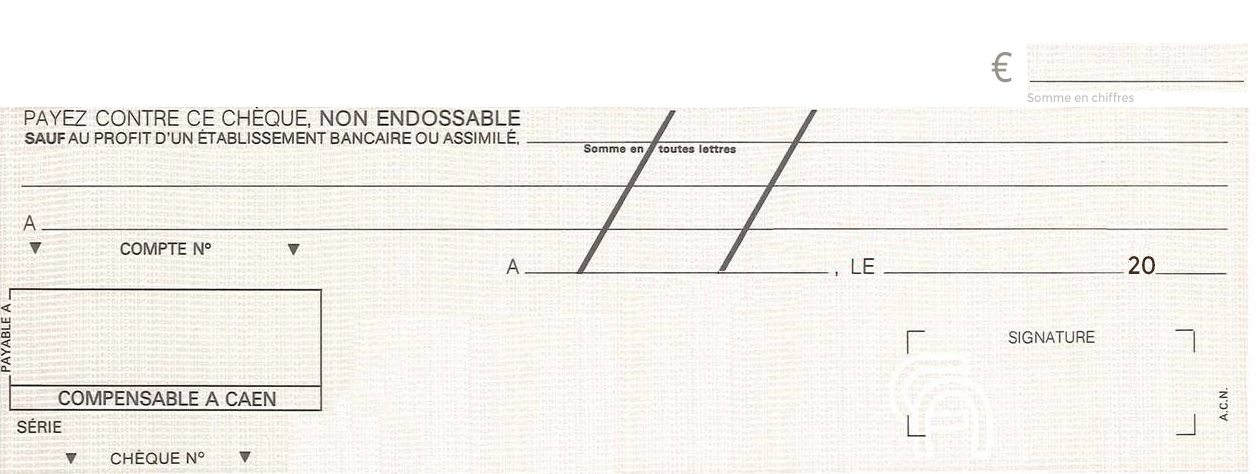
\includegraphics[scale=1]{FIG/spechequedebanque.jpg} 
 

\ExoCt{Représenter.}

Ranger dans l'ordre croissant les nombres : $3,35 \quad 3,53 \quad 3,55 \quad 3,05 \quad 3,353$
 


\ExoCt{Chercher. Communiquer.}

Éric a décomposé le nombre décimal  $E = 23\times 1000 + 6\times 10 + 4 +  5\times \dfrac{1}{1000} + 5\times \dfrac{1}{10} +  2\times 0,01 $. 

Peux-tu le retrouver ? $E = \ldots\ldots\ldots\ldots\ldots\ldots\ldots\ldots $

\ExoCt{Chercher. Communiquer.}

Le nombre $\dfrac{1}{3}$ est-il décimal ?
 
\ligne{3} 

\end{pageParcourst}



\begin{pageAuto} 

\ExoAuto

Entoure la ou les cases justes.


\begin{tabularx}{\linewidth}{|p{6cm}|X|X|X|X|}
\hline 
Énoncé & A & B & C & D \\ 
\hline 
$6$ est  & un chiffre &  un nombre & une lettre & Le double de 12 \\ 
\hline 
La partie décimale de 15,34 & 15 & 1534 & 0,34 & 34 \\ 
\hline
$124,07=$ & $\dfrac{12407}{100}$ &  $\dfrac{12,407}{100}$ &  $\dfrac{12407}{100}$ &  $\dfrac{12407}{10}$  \\ 
\hline 
Le chiffres des dixièmes de $13,457$ est  & $1$ & $3$ & $4$ & $5$ \\ 
\hline 
Lequel de ces nombres est compris entre $25,34$ et $25,40 $ & $25,034$ & $25,304$ & $25,341$ & $25,43$ \\ 
\hline 
 $2\times 10 +3\times 1+5\times 100 +\dfrac{6}{100}=$ & $2315,6$ &  $523,06$ &  $235,16$ &  $231,56$ \vspace{0.3cm} \\ 
\hline 
 $1342,04$ est compris entre & $1342$ et $1342,1$ &  $1342,3$ et  $1342,4$ & $1342,041$  et  $1342,042$&  $1342$ et $1343$ \\ 
\hline
\end{tabularx} 

\ExoAuto


 Le point $D$ et le point $O$ sont placés sur la droite graduée.
 


\definecolor{ffqqqq}{rgb}{1.,0.,0.}
\definecolor{wqwqwq}{rgb}{0.3764705882352941,0.3764705882352941,0.3764705882352941}
\definecolor{yqyqyq}{rgb}{0.5019607843137255,0.5019607843137255,0.5019607843137255}
\begin{tikzpicture}[line cap=round,line join=round,>=triangle 45,x=1.0cm,y=1.0cm]
\clip(1.4330456680992273,1.7995850535155078) rectangle (12.818294698183,2.4177546905415026);
\draw [color=yqyqyq](11.48969711916367,2.3930279050604626) node[anchor=north west] {$16,4$};
\draw [color=yqyqyq](1.590741496044137,2.3847856432334495) node[anchor=north west] {$16,3$};
\draw [line width=1.pt,color=wqwqwq] (2.,2.)-- (12.,2.);
\begin{scriptsize}
\draw [color=wqwqwq] (2.,2.)-- ++(-2.5pt,0 pt) -- ++(5.0pt,0 pt) ++(-2.5pt,-2.5pt) -- ++(0 pt,5.0pt);
\draw [color=wqwqwq] (3.,2.)-- ++(-2.5pt,0 pt) -- ++(5.0pt,0 pt) ++(-2.5pt,-2.5pt) -- ++(0 pt,5.0pt);
\draw [color=wqwqwq] (4.,2.)-- ++(-2.5pt,0 pt) -- ++(5.0pt,0 pt) ++(-2.5pt,-2.5pt) -- ++(0 pt,5.0pt);
\draw [color=wqwqwq] (5.,2.)-- ++(-2.5pt,0 pt) -- ++(5.0pt,0 pt) ++(-2.5pt,-2.5pt) -- ++(0 pt,5.0pt);
\draw [color=wqwqwq] (6.,2.)-- ++(-2.5pt,0 pt) -- ++(5.0pt,0 pt) ++(-2.5pt,-2.5pt) -- ++(0 pt,5.0pt);
\draw [color=wqwqwq] (7.,2.)-- ++(-2.5pt,0 pt) -- ++(5.0pt,0 pt) ++(-2.5pt,-2.5pt) -- ++(0 pt,5.0pt);
\draw [color=wqwqwq] (8.,2.)-- ++(-2.5pt,0 pt) -- ++(5.0pt,0 pt) ++(-2.5pt,-2.5pt) -- ++(0 pt,5.0pt);
\draw [color=wqwqwq] (9.,2.)-- ++(-2.5pt,0 pt) -- ++(5.0pt,0 pt) ++(-2.5pt,-2.5pt) -- ++(0 pt,5.0pt);
\draw [color=wqwqwq] (10.,2.)-- ++(-2.5pt,0 pt) -- ++(5.0pt,0 pt) ++(-2.5pt,-2.5pt) -- ++(0 pt,5.0pt);
\draw [color=wqwqwq] (11.,2.)-- ++(-2.5pt,0 pt) -- ++(5.0pt,0 pt) ++(-2.5pt,-2.5pt) -- ++(0 pt,5.0pt);
\draw [color=wqwqwq] (12.,2.)-- ++(-2.5pt,0 pt) -- ++(5.0pt,0 pt) ++(-2.5pt,-2.5pt) -- ++(0 pt,5.0pt);
\draw [color=wqwqwq] (2.5,2.)-- ++(-2.5pt,0 pt) -- ++(5.0pt,0 pt) ++(-2.5pt,-2.5pt) -- ++(0 pt,5.0pt);
\draw [color=wqwqwq] (3.5,2.)-- ++(-2.5pt,0 pt) -- ++(5.0pt,0 pt) ++(-2.5pt,-2.5pt) -- ++(0 pt,5.0pt);
\draw [color=ffqqqq] (4.5,2.)-- ++(-2.5pt,0 pt) -- ++(5.0pt,0 pt) ++(-2.5pt,-2.5pt) -- ++(0 pt,5.0pt);
\draw[color=ffqqqq] (4.561234103779965,2.1498811811635714) node {$D$};
\draw [color=wqwqwq] (5.5,2.)-- ++(-2.5pt,0 pt) -- ++(5.0pt,0 pt) ++(-2.5pt,-2.5pt) -- ++(0 pt,5.0pt);
\draw [color=wqwqwq] (6.5,2.)-- ++(-2.5pt,0 pt) -- ++(5.0pt,0 pt) ++(-2.5pt,-2.5pt) -- ++(0 pt,5.0pt);
\draw [color=wqwqwq] (7.5,2.)-- ++(-2.5pt,0 pt) -- ++(5.0pt,0 pt) ++(-2.5pt,-2.5pt) -- ++(0 pt,5.0pt);
\draw [color=wqwqwq] (8.5,2.)-- ++(-2.5pt,0 pt) -- ++(5.0pt,0 pt) ++(-2.5pt,-2.5pt) -- ++(0 pt,5.0pt);
\draw [color=ffqqqq] (9.5,2.)-- ++(-2.5pt,0 pt) -- ++(5.0pt,0 pt) ++(-2.5pt,-2.5pt) -- ++(0 pt,5.0pt);
\draw[color=ffqqqq] (9.55604435158216,2.1498811811635714) node {$O$};
\draw [color=wqwqwq] (10.5,2.)-- ++(-2.5pt,0 pt) -- ++(5.0pt,0 pt) ++(-2.5pt,-2.5pt) -- ++(0 pt,5.0pt);
\draw [color=wqwqwq] (11.5,2.)-- ++(-2.5pt,0 pt) -- ++(5.0pt,0 pt) ++(-2.5pt,-2.5pt) -- ++(0 pt,5.0pt);
\end{scriptsize}
\end{tikzpicture}

\vspace{0.2cm}

 Le point $D$ a pour abscisse $\ldots\ldots\ldots$ et le point $O$ a pour abscisse $\ldots\ldots\ldots$.
 
 
\ExoAuto

 Place sur la droite graduée le point A d'abscisse $23,5645$
 \vspace{0.2cm}
 
\definecolor{wqwqwq}{rgb}{0.3764705882352941,0.3764705882352941,0.3764705882352941}
\definecolor{yqyqyq}{rgb}{0.5019607843137255,0.5019607843137255,0.5019607843137255}
\begin{tikzpicture}[line cap=round,line join=round,>=triangle 45,x=1.0cm,y=1.0cm]
\clip(1.408318884694266,1.7171624352453752) rectangle (12.310052437048013,2.434239214195529);
\draw [color=yqyqyq](11.18969711916367,2.42 ) node[anchor=north west] {$23,57$};
\draw [color=yqyqyq](1.490741496044137,2.42) node[anchor=north west] {$23,56$};
\draw [line width=1.pt,color=wqwqwq] (2.,2.)-- (12.,2.);
\begin{scriptsize}
\draw [line width=1.6pt,color=yqyqyq] (2.,2.)-- ++(-2.5pt,0 pt) -- ++(5.0pt,0 pt) ++(-2.5pt,-2.5pt) -- ++(0 pt,5.0pt);
\draw [color=wqwqwq] (3.,2.)-- ++(-2.5pt,0 pt) -- ++(5.0pt,0 pt) ++(-2.5pt,-2.5pt) -- ++(0 pt,5.0pt);
\draw [color=wqwqwq] (4.,2.)-- ++(-2.5pt,0 pt) -- ++(5.0pt,0 pt) ++(-2.5pt,-2.5pt) -- ++(0 pt,5.0pt);
\draw [color=wqwqwq] (5.,2.)-- ++(-2.5pt,0 pt) -- ++(5.0pt,0 pt) ++(-2.5pt,-2.5pt) -- ++(0 pt,5.0pt);
\draw [color=wqwqwq] (6.,2.)-- ++(-2.5pt,0 pt) -- ++(5.0pt,0 pt) ++(-2.5pt,-2.5pt) -- ++(0 pt,5.0pt);
\draw [color=wqwqwq] (7.,2.)-- ++(-2.5pt,0 pt) -- ++(5.0pt,0 pt) ++(-2.5pt,-2.5pt) -- ++(0 pt,5.0pt);
\draw [color=wqwqwq] (8.,2.)-- ++(-2.5pt,0 pt) -- ++(5.0pt,0 pt) ++(-2.5pt,-2.5pt) -- ++(0 pt,5.0pt);
\draw [color=wqwqwq] (9.,2.)-- ++(-2.5pt,0 pt) -- ++(5.0pt,0 pt) ++(-2.5pt,-2.5pt) -- ++(0 pt,5.0pt);
\draw [color=wqwqwq] (10.,2.)-- ++(-2.5pt,0 pt) -- ++(5.0pt,0 pt) ++(-2.5pt,-2.5pt) -- ++(0 pt,5.0pt);
\draw [color=wqwqwq] (11.,2.)-- ++(-2.5pt,0 pt) -- ++(5.0pt,0 pt) ++(-2.5pt,-2.5pt) -- ++(0 pt,5.0pt);
\draw [line width=1.6pt,color=yqyqyq] (12.,2.)-- ++(-2.5pt,0 pt) -- ++(5.0pt,0 pt) ++(-2.5pt,-2.5pt) -- ++(0 pt,5.0pt);
\draw [color=wqwqwq] (2.5,2.)-- ++(-2.5pt,0 pt) -- ++(5.0pt,0 pt) ++(-2.5pt,-2.5pt) -- ++(0 pt,5.0pt);
\draw [color=wqwqwq] (3.5,2.)-- ++(-2.5pt,0 pt) -- ++(5.0pt,0 pt) ++(-2.5pt,-2.5pt) -- ++(0 pt,5.0pt);
\draw [color=wqwqwq] (4.5,2.)-- ++(-2.5pt,0 pt) -- ++(5.0pt,0 pt) ++(-2.5pt,-2.5pt) -- ++(0 pt,5.0pt);
\draw [color=wqwqwq] (5.5,2.)-- ++(-2.5pt,0 pt) -- ++(5.0pt,0 pt) ++(-2.5pt,-2.5pt) -- ++(0 pt,5.0pt);
\draw [color=wqwqwq] (6.5,2.)-- ++(-2.5pt,0 pt) -- ++(5.0pt,0 pt) ++(-2.5pt,-2.5pt) -- ++(0 pt,5.0pt);
\draw [color=wqwqwq] (7.5,2.)-- ++(-2.5pt,0 pt) -- ++(5.0pt,0 pt) ++(-2.5pt,-2.5pt) -- ++(0 pt,5.0pt);
\draw [color=wqwqwq] (8.5,2.)-- ++(-2.5pt,0 pt) -- ++(5.0pt,0 pt) ++(-2.5pt,-2.5pt) -- ++(0 pt,5.0pt);
\draw [color=wqwqwq] (9.5,2.)-- ++(-2.5pt,0 pt) -- ++(5.0pt,0 pt) ++(-2.5pt,-2.5pt) -- ++(0 pt,5.0pt);
\draw [color=wqwqwq] (10.5,2.)-- ++(-2.5pt,0 pt) -- ++(5.0pt,0 pt) ++(-2.5pt,-2.5pt) -- ++(0 pt,5.0pt);
\draw [color=wqwqwq] (11.5,2.)-- ++(-2.5pt,0 pt) -- ++(5.0pt,0 pt) ++(-2.5pt,-2.5pt) -- ++(0 pt,5.0pt);
\end{scriptsize}
\end{tikzpicture}



\end{pageAuto}


\begin{pageBrouillon} 
 
\ligne{30}

\end{pageBrouillon}
